\chapter{Study of A/H$\rightarrow\tau\tau\rightarrow$two jets}

\section{Introduction}
Discovery of the heavy neutral Higgs boson would be an important verification of the MSSM Higgs sector and hence the MSSM itself. If calculated its mass could be used as part of a global fit to determine all MSSM parameters. 

Negative searches for the Higgsstrahlung process $e^{+}e^{-} \rightarrow Zh/ZH$ and $e^{+}e^{-} \rightarrow Ah/AH$ at LEP2 yielded limits of $m_{h,H}$\,$>$\,93\GeVcc~\cite{Schael:2006cr}. A $\tan{\beta}$ range could only be excluded within the context of a particular MSSM scenario. The \mhmax benchmark scenario, see Section~\ref{sec:mssm} where m$\mathrm{_h \approx 130\GeVcc}$ and $\mathrm{m_A \gg m_h}$, provided the most conservative $\tan{\beta}$ exclusion of 0.7\,$>$\,$\mathrm{\tan{\beta}}$\,$>$\,2.0 for top quark mass ($\mathrm{m_{t}}$)\,=\,174.3\GeVcc~\cite{Schael:2006cr}. The Tevatron placed upper limits on the \plane plane, which are shown together with the LEP2 limits in Figure~\ref{fig:lep_limit}.

\begin{figure}[htb]
\centering
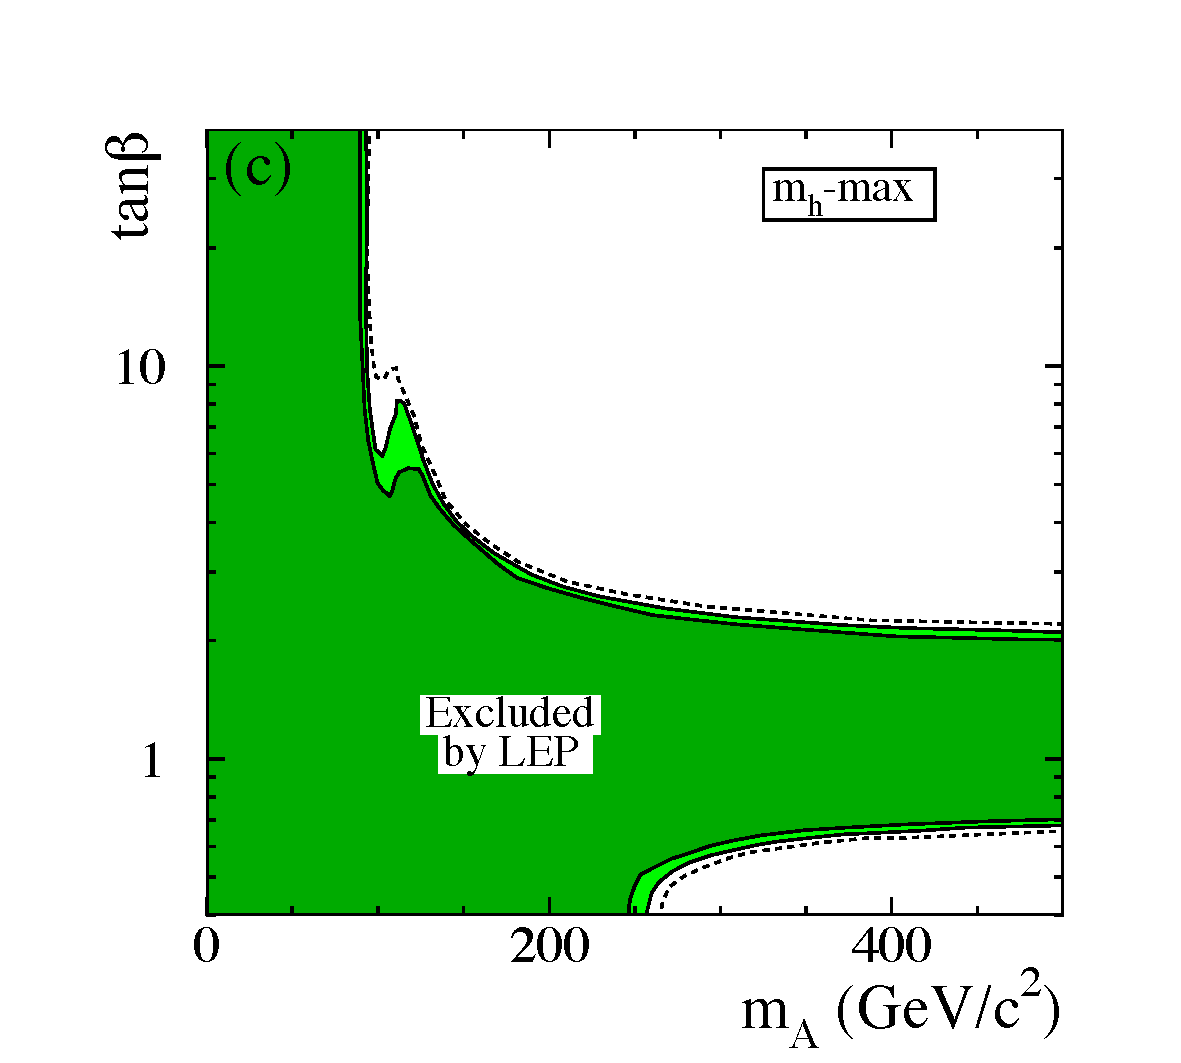
\includegraphics[width=0.47\textwidth]{analysis/matbmax_col}
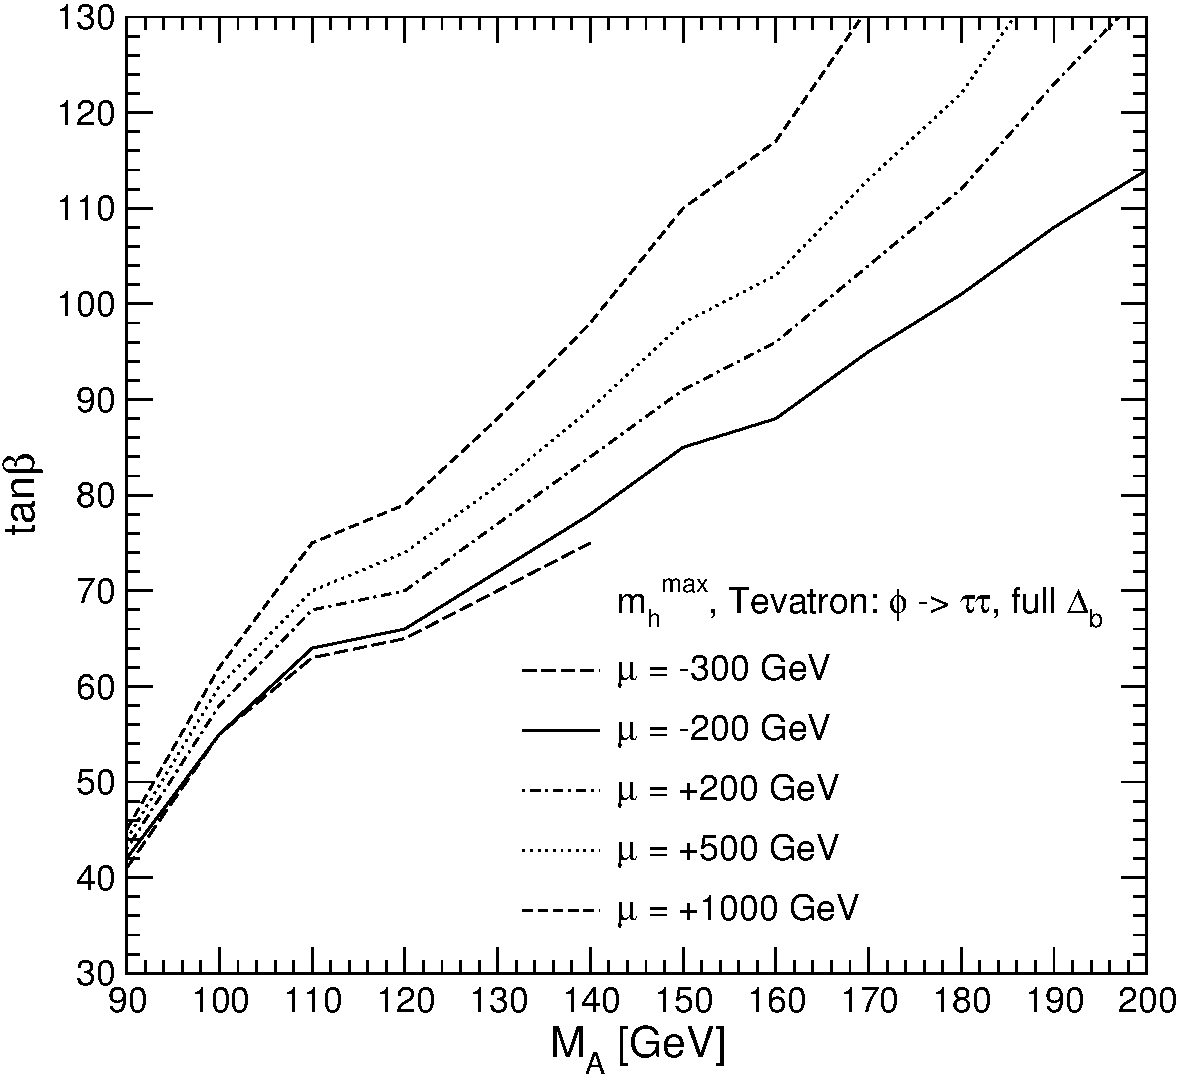
\includegraphics[width=0.45\textwidth]{analysis/t4l-benchP16}
\caption{LEP2 (left) and Tevatron (right) limits in the $\tan{\beta}$ - $m_{A}$ plane for the $\mhmax$ scenario.~\cite{Schael:2006cr, citeulike:894146}  
\label{fig:lep_limit}}
\end{figure}

\begin{figure}[htb]
\centering
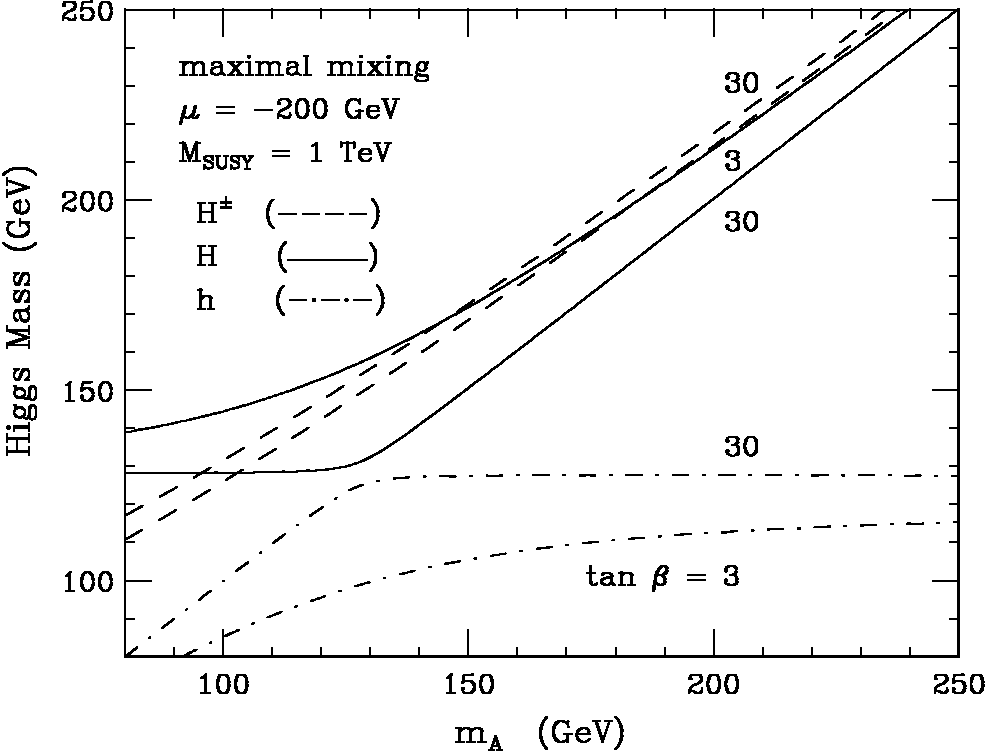
\includegraphics[width=0.55\textwidth]{analysis/hhmasses}
\caption{Masses of the Higgs bosons for two possible values of $\tan{\beta}$ as a function of $m_{A}$ in the \mhmax scenario.~\cite{citeulike:888485}  
\label{fig:Higgs_degenerate}}
\end{figure}

It is common for an MSSM search to be conducted with a set of benchmark parameters. The scenario that provides the most conservative $\tan{\beta}$ reach is the \mhmax scenario. This scenario was described Chapter 7 and occurs when $m_A \gg \mhmax$. In this scenario the light scalar, h, reaches its maximal value of $\sim$\,130\GeVcc and the neutral heavy Higgs bosons, $A$ and $H$, become almost degenerate in mass, this is shown in Figure~\ref{fig:Higgs_degenerate}. The mass difference between the two is within CMS's jet resolution, thus the two signal distributions are combined in searches.

%Due to the enhanced Yukawa coupling to down type fermions previous CMS studies have studied the decays $H/A \rightarrow \mu^{+}\mu^{-}$, $H/A \rightarrow \tau^{+}\tau{-}$ and $H/A \rightarrow b\bar{b}$ for the associated production channel $gg \rightarrow b\bar{b}H/A$~\cite{CMS_TDR_PHYS_vol2}.
%FIXME check all channels in TDR - also ref summary of the CMS potential...

\begin{figure}[!Hhtb]
\centering
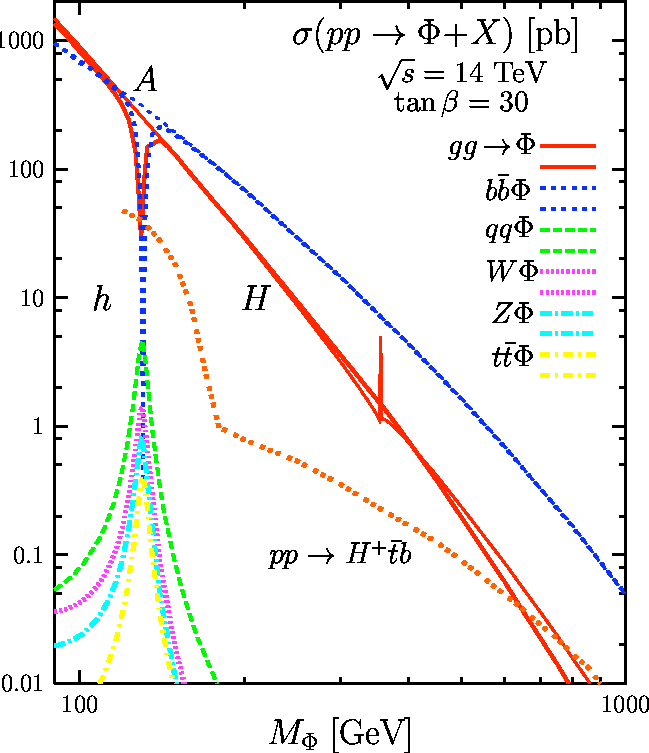
\includegraphics[width=0.45\textwidth]{analysis/xslhc-all}
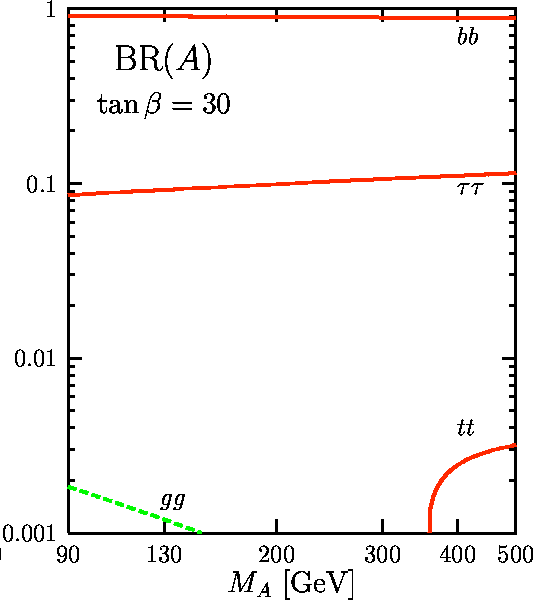
\includegraphics[width=0.45\textwidth]{analysis/bra-mssm}
\caption{Cross section for MSSM Higgs boson production (left) and branching ratio of the $A$ (right) at the LHC for $\tan{\beta}=30$.~\cite{citeulike:888485}  
\label{fig:Higgs_xsection_BR}}
\end{figure}

Figure~\ref{fig:Higgs_xsection_BR} shows the $H/A$ cross-sections and $A$ branching ratio (BR) for the \mhmax scenario with $\tan{\beta} = 30$. Decays to b quarks and $\tau$'s dominate due to the enhanced coupling to heavy down-type quarks, see Table~\ref{tab:MSSMcoupling}. Similar branching ratios are also obtained for the $H$. The dominant decay to b quarks would be difficult to search for with CMS due to the large hadronic background at the LHC. Thus the second most common decay, to 2 $\tau$ leptons, was studied.

%The $\mu$ decays (not shown in plot) were useful for $m_{A} < 300 \GeVcc$. For large values of $m_{A}$ the $\tau$ channel was favoured.

Many $\tau$ decay channels have been studied at CMS~\cite{CMS_TDR_PHYS_vol2} with fully hadronic final states, with $\tau \rightarrow \nu + j$ providing the highest $m_{A}$ reach. This channel relies on the production associated with b quarks~\cite{CMS_TDR_PHYS_vol2, citeulike:903864} (Figure~\ref{fig:feynman}) and uses $\tau$ and b-tagging for event selection. It was decided for this study to investigate the possibility of replacing the b-tagging selection with one based on \MET. With the elimination of b-tagging this analysis was also sensitive to the second most common production mechanism, \ggH (Figure~\ref{fig:feynman}). The study was performed for the three sample values of $m_A$ = 200, 500 and 800 \GeVcc. This analysis is described below and the resulting reach in the \plane plane for the \mhmax scenario presented.

\begin{figure}
	\centering
	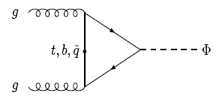
\includegraphics[width=0.35\textwidth]{analysis/feynman-associated}
	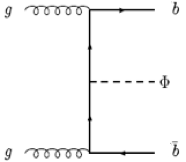
\includegraphics[width=0.25\textwidth]{analysis/feynman-fusion}
	\caption{Feynman diagrams of the major Higgs production mechanisms studied in this analysis. Gluon-gluon fusion is shown on the left and associated b production on the right.\label{fig:feynman}}
\end{figure}


\section{Signal and background generation}
Until CMS data-taking begins Monte Carlo data has to be used. Events were produced with full detector simulation at an instantaneous luminosity of \lowlumi. Signal events were generated with PYTHIA~\cite{citeulike:903853} procesess 181 (\bbH) and 152 (\ggH) for 3 values of $\mathrm{m_{A}}$: 200, 500 and 800 \GeVcc. Backgrounds included events with $\tau$ jets and those with jets, or electrons, which could be mis-tagged as a $\tau$. PYTHIA-generated backgrounds included QCD multi-jets, \ZTauTau, \Zee, \TopTop, \Wtb\xspace and \Wjet. W bosons in the samples \TopTop, \Wjet\xspace and \Wtb were forced to decay $W \rightarrow \tau\nu$. All $\tau$ decays were forced to hadrons with the TAUOLA package~\cite{citeulike:903857}.

%PT bins etc...

Loose cuts were applied to the background samples at the generator level to avoid generating excess events that would not pass the offline selection. These selections were looser than those used offline. The main requirement was for 2 $\tau$-like jets with generated \PT (\pthat)\,$>$\,50\GeV. A jet was formed with the PYTHIA PYCELL routine and tagged as $\tau$-like if it was within the tracker acceptance, $|\eta|$\,$<$\,2.4, and had at least one stable charged particle with \PT$>$\,30\GeVc. No \PT preselection was applied to the \ZTauTau sample. A cut of $\mathrm{M_{ee}}$\,$>$\,15\GeVcc was applied to the \Zee sample. No preselection was applied to the signal samples. The generated number of events and generator cut efficiency, $\epsilon_{kine}$, for all generated datasets are shown in Table~\ref{table:datasets}.

\begin{table}[htb]
	\centering
\begin{tabular}{|l|c|c|c|c|}
\hline
sample & $\sigma\times$ BR & generated & generated & $\epsilon_{kine}$ \\ 
        & (fb)              & luminosity (\fb) & events & \\ \hline                      
\bbH\,$m_A = 200 \GeVcc$ & - & - & 100K & 1\\ \hline
\bbH\,$m_A = 500 \GeVcc$ & - & - & 100K & 1\\ \hline
\bbH\,$m_A = 800 \GeVcc$ & - & - & 100K & 1\\ \hline
\ggH\,$m_A = 200 \GeVcc$ & - & - & 100K & 1\\ \hline
\ggH\,$m_A = 500 \GeVcc$ & - & - & 100K & 1\\ \hline
\ggH\,$m_A = 800 \GeVcc$ & - & - & 100K & 1\\ \hline
QCD\,$50 < \pthat < 80\GeV$ & $2.11\ten{10}$ & 0.020 & 100K & 2.44\ten{-4} \\ \hline
QCD\,$80 < \pthat < 120\GeV$ & $2.94\ten{9}$ & 0.012 & 200K & 5.77\ten{-3} \\ \hline
QCD\,$120 < \pthat < 170\GeV$ & $5.03\ten{8}$ & 0.009 & 200K & 4.19\ten{-2} \\ \hline
QCD\,$170 \GeV < \pthat$ & $1.33\ten{8}$ & 0.008 & 1000K & 2.12\ten{-1} \\ \hline
\Ztautau\,\ZTauTaua & $1.57\ten{6}$ & 4.3 & 128K & 1.90\ten{-2}\\ \hline
\Ztautau\,\ZTauTaub & $1.24\ten{4}$ & 59 & 70K & 9.53\ten{-2} \\ \hline
\Ztautau\,\ZTauTauc & $6.22\ten{2}$ & 299 & 60K & 3.23\ten{-1} \\ \hline
\Zee & 3.96\ten{6} & 0.24 & 985K & 1\\ \hline
\TopTop & 5.76\ten{3} & 285 & 80K & 4.88\ten{-2}\\ \hline
\Wjet & 5.74\ten{5} & 32 & 400K & 2.16\ten{-2} \\ \hline
\Wtb & 7.10\ten{2} & 3053 & 30K & 1.38\ten{-2}\\ \hline
%$S/\sqrt{B}$ & 6.2 & 7.8 & 5.5 \\ \hline
\end{tabular}
\caption{Generated datasets listing the process cross section, generation cut efficiency, generated events and luminosity. Luminosity and cross sections are not shown for the signal samples as they cannot be calculated without knowledge of the MSSM parameters.  Background cross sections are assumed to have no error. Errors on the number of background events are introduced later for the dominant backgrounds.\label{table:datasets}}
\end{table}

%All samples were produced with full detector simulation at an instantaneous luminosity of \lowlumi.

%\subsection{Kinematics}
%not sure if needed

\section{Level-1 and high level triggers}
The Level-1 $\tau$ trigger was described in Section~\ref{sec:trigger}. Either a single 93\GeV or two 66\GeV $\tau$ triggers were required. These values were optimised for the available trigger bandwidth, 3.2 kHz, as shown in Ref~\cite{CMS_TDR_PHYS_vol1}. The \ET cut was applied after Level-1 jet corrections. These corrections were optimised for non $\tau$ jets and thus over-corrected the $\tau$ \ET. The signal efficiency and purity as a function of $\tau$ \ET can be seen in Figure~\ref{fig:L1_eff_purity}.\footnote{This analysis uses the \ET jet recombination scheme that results in massless jets where \PT is equivalent to \ET.}

\begin{figure}[tb]
\centering
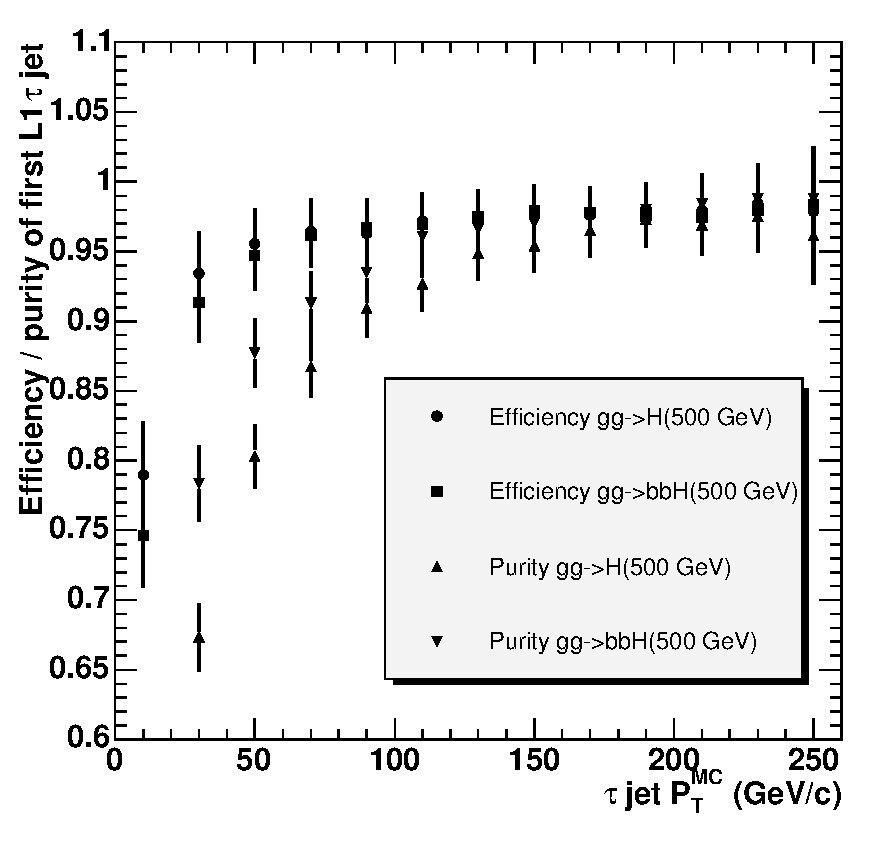
\includegraphics[width=0.49\textwidth]{analysis/L1Tau1Eff_vs_Et}
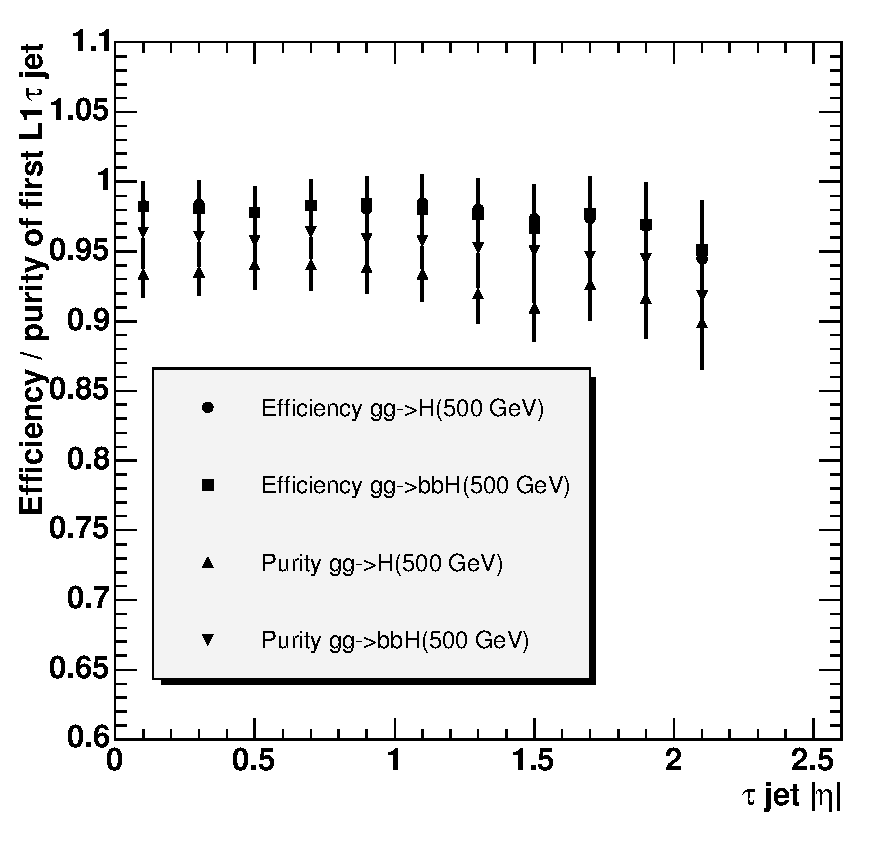
\includegraphics[width=0.49\textwidth]{analysis/L1Tau1Eff_vs_Eta}
\caption{Level-1 efficiency (ratio of Level-1 to Monte carlo level $\tau$s) and purity of the most energetic $\tau$. A $\tau$ is defined as pure if it is within a distance of 0.4 in R of the true jet.   
\label{fig:L1_eff_purity}}
\end{figure}

The HLT strategy was described in section~\ref{sec:CaloPxl}. The event selection criteria required two HLT $\tau$ candidates with no jet \ET threshold. No \ET threshold was applied as the Level-1 threshold had already been applied and the $\tau$ id criteria resulted in an adequate rate of 4 Hz.

\section{Offline reconstruction and selections}
The offline process included: further $\tau$ identification with tighter cuts: jet calibration and cuts; \MET calibration and cuts; and Higgs boson reconstruction. These cuts were optimised for the greatest 5$\sigma$ discovery reach in the \plane plane for each of the 3 $m_A$ scenarios. 

\subsection{$\tau$ Identification and reconstruction}
The two HLT $\tau$ candidates were reconstructed with the iterative cone algorithm~\cite{CMS_TDR_PHYS_vol1} and cone size 0.4. The algorithm took as input calorimeter towers with thresholds of \ET\,=\,0.5\GeV and E\,=\,0.8\GeV with a 1\GeV seed threshold. These cuts had been optimised to suppress fake jet contamination~\cite{citeulike:903868}. Global track reconstruction was performed with the full tracker and parameters listed in Section~\ref{sec:tracker_isolation}.

%Initial $\tau$ identification was applied with loose cuts which were then individually tightened. Candidates were required to have a lead track within the matching cone, $R_{m} = 0.1$, with $\PT > 10 \GeVc$ 

The following offline $\tau$ id cuts were applied: jet \ET, tracker isolation and electron rejection.

\subsubsection{$\tau$ jet threshold}
$\tau$ jet \ET thresholds were used to reduce the backgrounds. Figure~\ref{fig:tau_max_min} shows the signal \ET distribution. The difference between the \ET of the two $\tau$ jets motivated the use of asymmetric \ET cuts. The least energetic $\tau$ was required to have $\ET > 50 \GeV$ due to the background preselection. The most energetic $\tau$ \ET cut was set to 65, 100 and 130 \GeV for the three $m_{A}$ scenarios. 

\begin{figure}[tb]
\centering
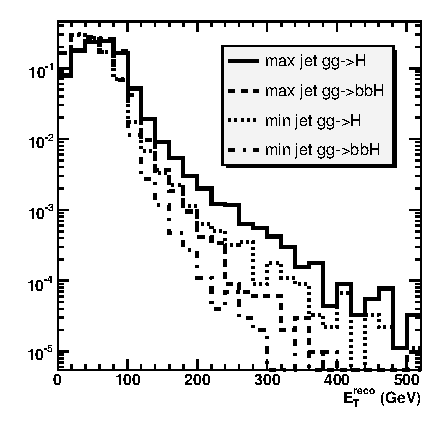
\includegraphics[width=0.45\textwidth]{analysis/TauEt_max_min_200}
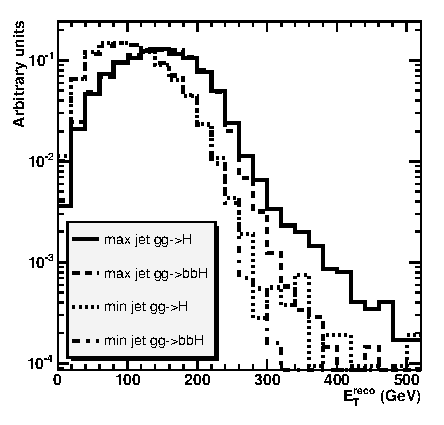
\includegraphics[width=0.45\textwidth]{analysis/TauEt_max_min_500}
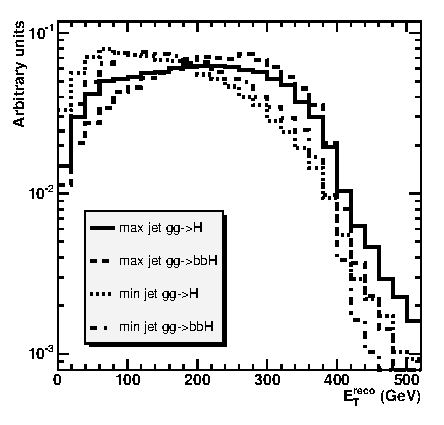
\includegraphics[width=0.45\textwidth]{analysis/TauEt_max_min_800}
\caption{$E_{T}^{\mathrm{reco}}$ distribution for signal datasets, $m_{A}=200$\GeVcc (left), $m_{A}=500$\GeVcc (right) and $m_{A}=800$\GeVcc (bottom).   
\label{fig:tau_max_min}}
\end{figure}

\subsubsection{Tracker isolation}
Tracks reconstructed with the full tracker were used to recalculate the tracker isolation. The parameters were the same as those at the HLT, with the exceptions $\mathrm{p_{T}^{ltr} > 32 \GeV}$ and $\mathrm{R_{s}=0.04}$. This was done to further reduce the QCD fake rate for this particular analysis. Also a requirement on the number of signal tracks was introduced. The effect of this can be seen in Figure~\ref{fig:sig_cone}, where the number of tracks within the signal cone around the lead track is shown for the main data samples. It can be seen that a requirement for one signal track rejects 60--70\% of the QCD multi-jet background.

\begin{figure}[tb]
\centering
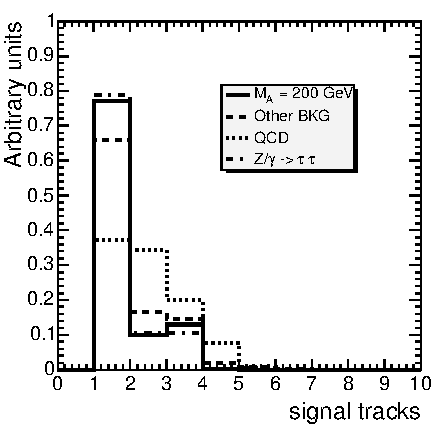
\includegraphics[width=0.45\textwidth]{analysis/TauProngs_200}
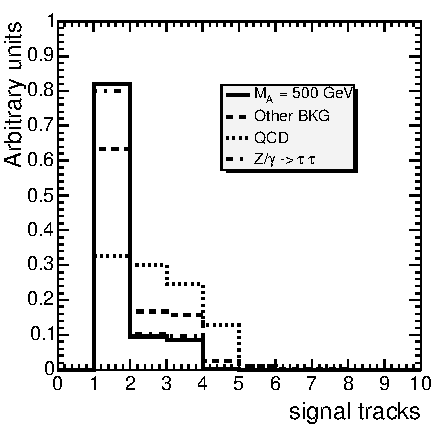
\includegraphics[width=0.45\textwidth]{analysis/TauProngs_500}
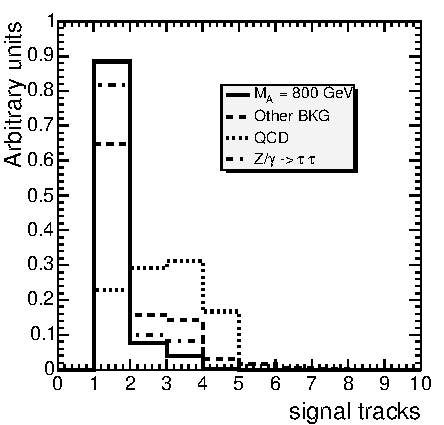
\includegraphics[width=0.45\textwidth]{analysis/TauProngs_800}
\caption{Signal track distribution for signal, QCD multi-jets, \Ztautau\xspace and other backgrounds for $m_{A}=200$\GeVcc (left), $m_{A}=500$\GeVcc (right) and $m_{A}=800$\GeVcc (bottom).\label{fig:sig_cone}}
\end{figure}

%\begin{table}[tbp]
%	\begin{tabular}{|l|c|c|c|c|}
%	\hline
%	& $m_{A}=200 \GeVcc$ & QCD multi-jets & \Ztautau & S/$\sqrt(\rm B)$ \\ \hline
%	1 or 3 tracks, $R_{s}=0.04$ & 38.1 & 61.8 & 8.5 & 4.5 \\ \hline
%	1 track, $R_{s}=0.04$ & 35.3 & 23.9 & 4.2 & 6.6 \\ \hline
%	1 or 3 tracks, $R_{s}=0.07$ & 38.4 & 109.6 & 8.5 & 2.5 \\ \hline
%	1 track, $R_{s}=0.07$ & 35.3 & 24.0 & 4.2 & 6.6 \\ \hline
 %   \end{tabular}
%\caption{Expected number of events and signal significance within $m_{A}=200\GeVcc$ mass window (defined later) for 60 \fb of data in the \mhmax scenario with $\tan{\beta}=20$.\label{tab:tracks}}
%\end{table} 

\subsubsection{Electron rejection}
To reduce \Zee\xspace contamination a cut on the hottest HCAL tower in the jet was introduced, as described in Section~\ref{sec:e_rejection}. Both $\tau$ jet candidates were required to pass the threshold. Figure~\ref{fig:lowHotHcal} shows the least hot HCAL tower of the two reconstructed $\tau$s in an event. A cut of 1.5 \GeV was sufficient to suppress highly \Zee\xspace.

\begin{figure}[!Hhtb]
\centering
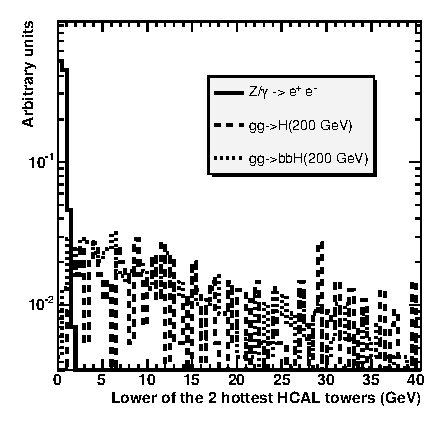
\includegraphics[width=0.45\textwidth]{analysis/lowestHottestHCALtower}
\caption{Distribution of the lowest value of the 2 $\tau$ jets hottest HCAL tower. All samples have passed both trigger levels and the offline tracker isolation.\label{fig:lowHotHcal}}
\end{figure}

Previous studies~\cite{CMS_TDR_PHYS_vol2} have shown further $\tau$ tagging procedures developed at CMS based on impact parameter and the $\tau$ mass did not provide significant improvement after the trigger and offline tracker isolation.

\subsubsection{$\tau$ \ET calibration}
The $\tau$ jets were calibrated with the Monte Carlo jet \ET corrections in Section~\ref{sec:MC_tau_calib}. Figure~\ref{fig:analysis_tau_scale} shows the effect of the correction. The overcorrection in the first \ET bin of the left plot was due to the application of tighter cuts than for the calibration. The overcorrection was not large enough to warrant a new calibration.

\begin{figure}[!Hhtb]
\centering
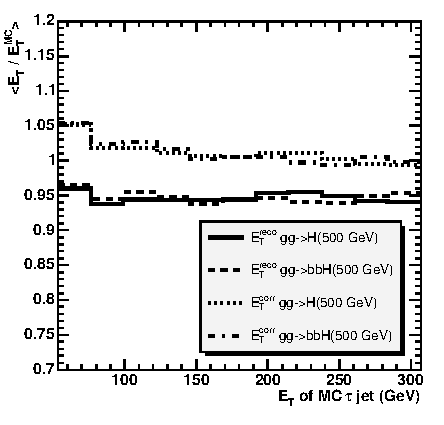
\includegraphics[width=0.45\textwidth]{analysis/TauEtScale_vs_Et}
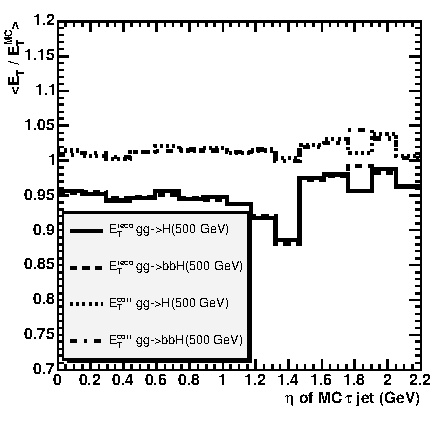
\includegraphics[width=0.45\textwidth]{analysis/TauEtScale_vs_Eta}
\caption{$E_{T}$ distribution and calibration for signal events passing cuts $\mathrm{E_{T}^{reco} > 50} \GeV, \mathrm{p_{T}^{ltr}} > 32 \GeVc$.\label{fig:analysis_tau_scale}}
\end{figure}

\subsection{Missing energy}
The \MET for an event was measured by summing all the calorimeter towers and obtaining $\mathrm{E_{x}}$ and $\mathrm{E_{y}}$. True (MC) \MET was calculated by summing all stable Monte Carlo particles except $\nu$ and $\mu$. The true \MET distributions can be seen in Figure~\ref{fig:MET} along with the difference between the true and reconstructed \MET. It can be seen that the detector \MET for the multi-jet background was considerably higher than the true value. This was due to limits on the detector's coverage and the imperfect calorimeter response.

\begin{figure}[!Hhtb]
\centering
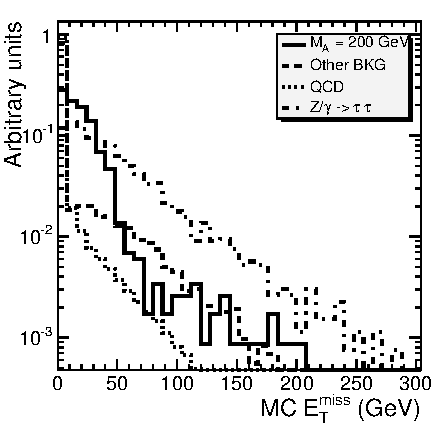
\includegraphics[width=0.45\textwidth]{analysis/MCMET_200}
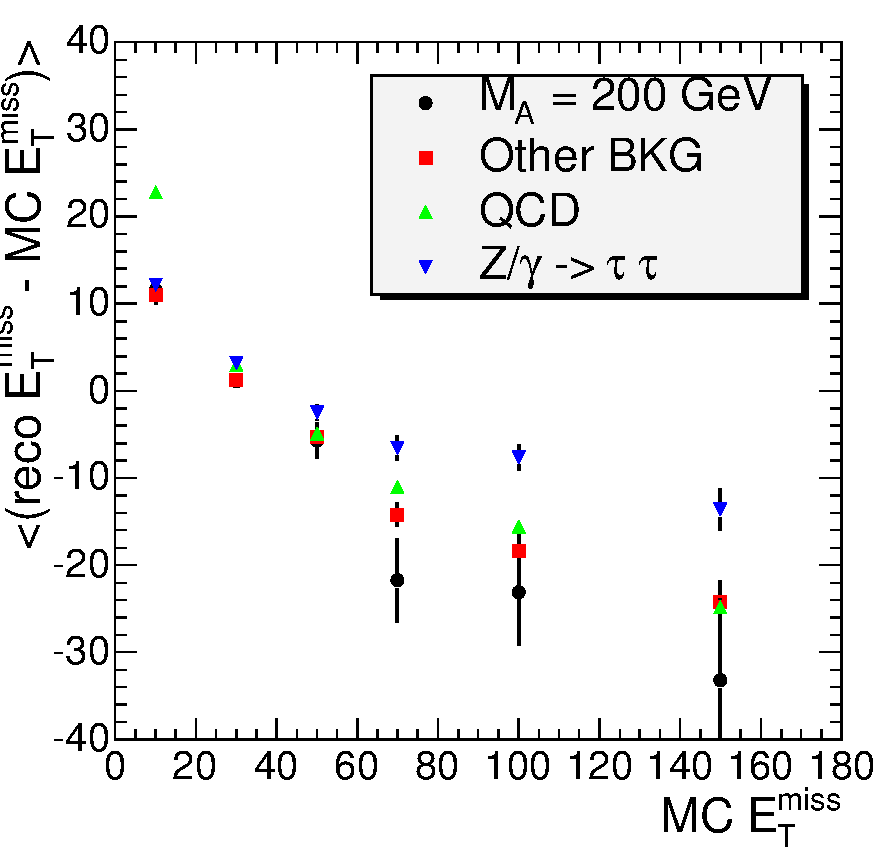
\includegraphics[width=0.45\textwidth]{analysis/MET_profile_200}
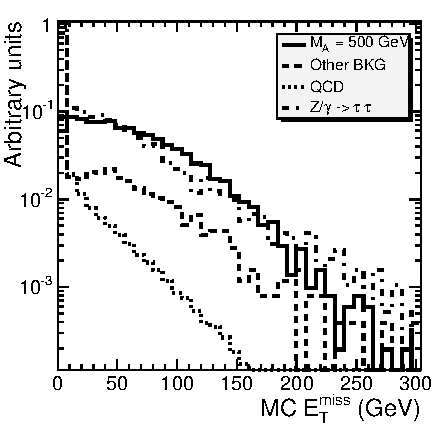
\includegraphics[width=0.45\textwidth]{analysis/MCMET_500}
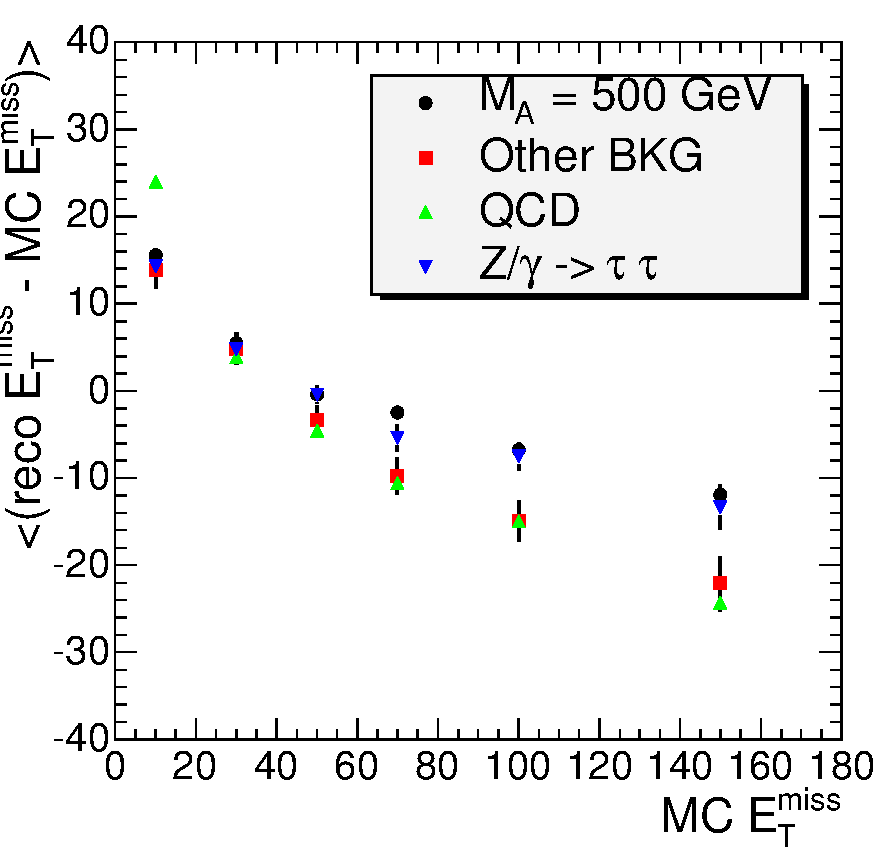
\includegraphics[width=0.45\textwidth]{analysis/MET_profile_500}
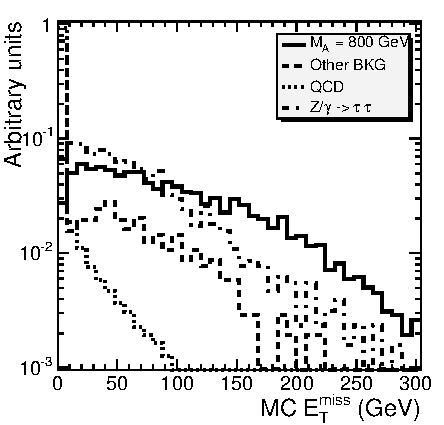
\includegraphics[width=0.45\textwidth]{analysis/MCMET_800}
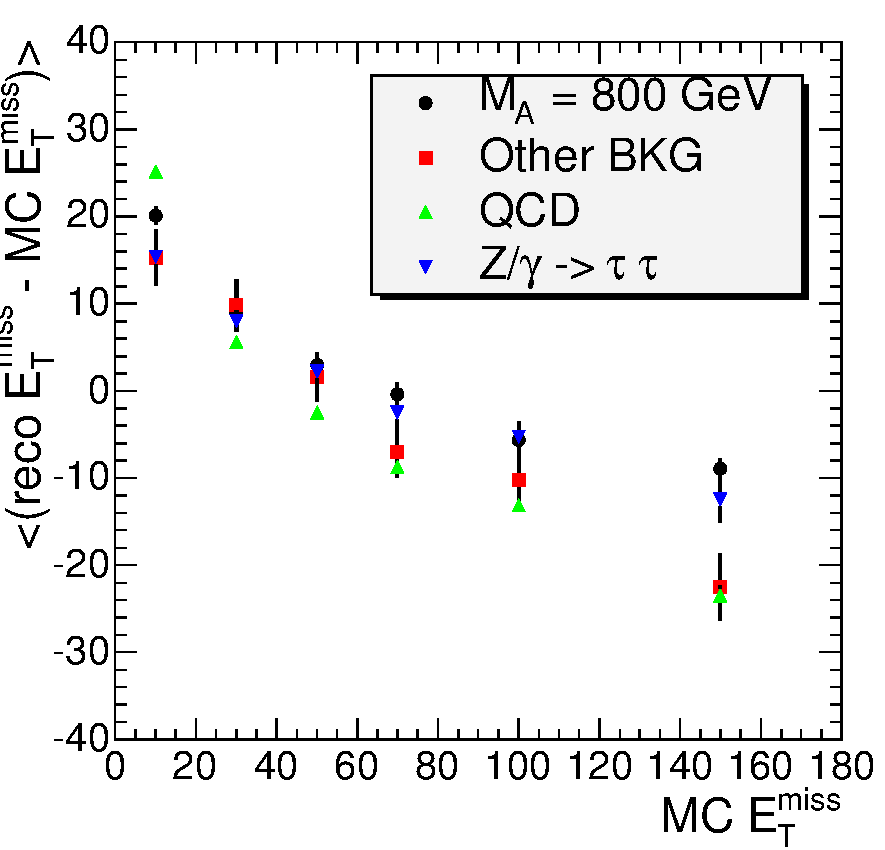
\includegraphics[width=0.45\textwidth]{analysis/MET_profile_800}
\caption{True \MET distribution (left) and difference between true and reconstructed \MET (right) for $m_{A}=200$\GeVcc (top), $m_{A}=500$\GeVcc (middle) and $m_{A}=800$\GeVcc (bottom). The background distributions differ between the $m_A$ plots as different cuts are applied for each scenario.\label{fig:MET}}
\end{figure}

Calibrations for the detector \MET response had been developed~\cite{citeulike:905600}. These corrections involved a global jet reconstruction for jets with \ET\,$>$\,25\GeV. For each jet the constituent towers energy contributions were replaced by that of the jet. The jet energy was calibrated to correct for out-of-cone energy leakage and pileup. The correction may be written:

\begin{equation}
\rm E_{\rm Tx(y)}^{\rm miss}= -(\rm E _{Tx(y)}^{\rm raw}+
                           \sum _{jets} (\rm E _{\rm Tx(y)}^{\rm corr.jet} - \rm E _{\rm Tx(y)}^{\rm raw jet}))
\label{eqn:MET_corr}
\end{equation}

where $\rm E _{Tx(y)}^{\rm raw}, \rm E _{\rm Tx(y)}^{\rm corr.jet} \mathrm{ and }\,\rm E _{\rm Tx(y)}^{\rm raw jet}$ represent the calorimeter response, corrected and uncorrected jet energies, respectively. 

\begin{figure}[!Hhtb]
\centering
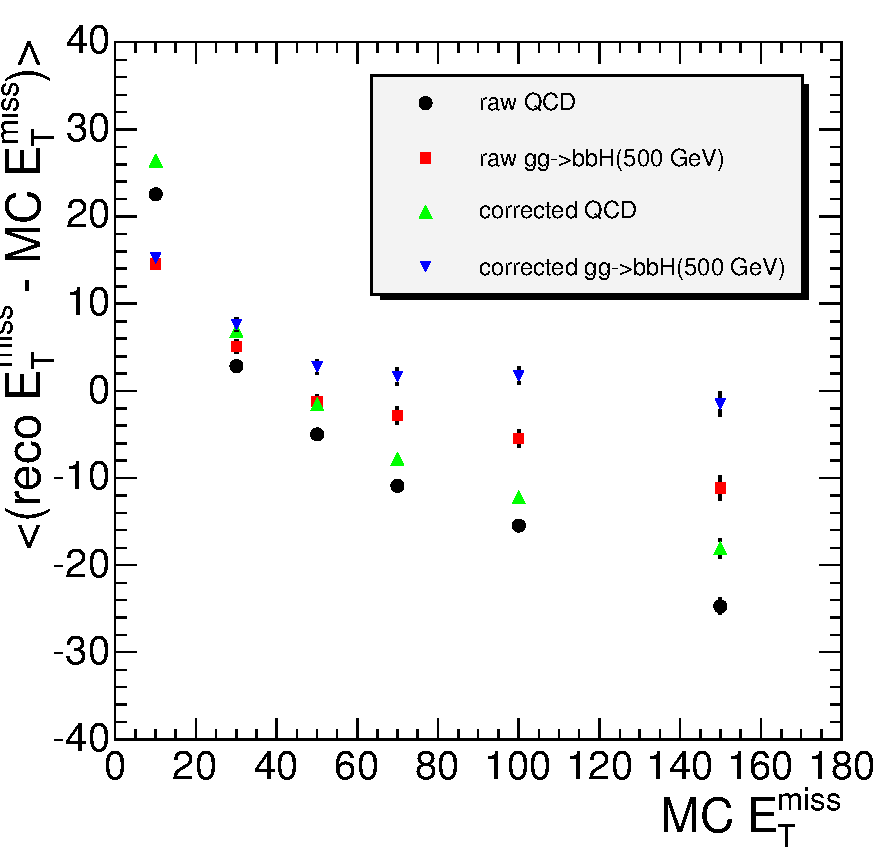
\includegraphics[width=0.45\textwidth]{analysis/MET_profile}
\caption{Average difference between reconstructed and true \MET (GeV) in QCD and $gg \rightarrow bbH$ events, both with and without corrections applied.\label{fig:MET_profile}}
\end{figure}

Figure~\ref{fig:MET_profile} shows the effect of the \MET correction. For events with true (MC) $\MET < 40 \GeV$ the correction can be seen to overestimate the \MET of the multi-jet sample while providing a negligible correction to the Higgs events. Thus the correction was only applied to events with $\MET > 40 \GeV$.

The \MET cut was set to 50, 70 and 70\GeV for $m_{A} = 200, 500 \mathrm{\,and\,} 800\GeVcc$, respectively. The $m_{A} = 200 \GeVcc$ cut had a low signal efficiency ($\sim$\,10\%) but was necessary for background suppression.

\subsection{Higgs mass reconstruction}
The undetectable neutrinos required assumptions to be made to allow the Higgs boson mass to be reconstructed. It was assumed that the $\nu$ was emitted collinear with the $\tau$. The corrected \MET could then be projected onto the two jet direction vectors. This then allowed the reconstructed Higgs mass, $\mathrm{M_{\tau \tau}}$, to be derived with:

\begin{equation}
	\mathrm{ M_{\tau \tau} = [2\,E_{\tau 1}\,E_{\tau 2} ( 1 - \cos{\theta_{\tau \tau}})]^{1/2} }
\end{equation}

where $\mathrm{E_{\tau 1},\,E_{\tau 2},\,\cos{\theta_{\tau \tau}}}$ represent the \ET of the two $\tau$s and the angle in $\theta$ between them. 

A number of quality cuts were applied to improve the $M_{\tau\tau}$ resolution. These requirements were positive energy neutrinos and non-back-to-back $\tau$ jets. Figure~\ref{fig:mass_resolution} shows the $M_{\tau\tau}$ distribution as a function of the angle in $\phi$ between the jets, $\Delta \phi_{jj}$, and as each reconstruction cut was applied. The $\Delta \phi_{jj}$ cut was set to 175\de.

\begin{figure}[!Hhtb]
\centering
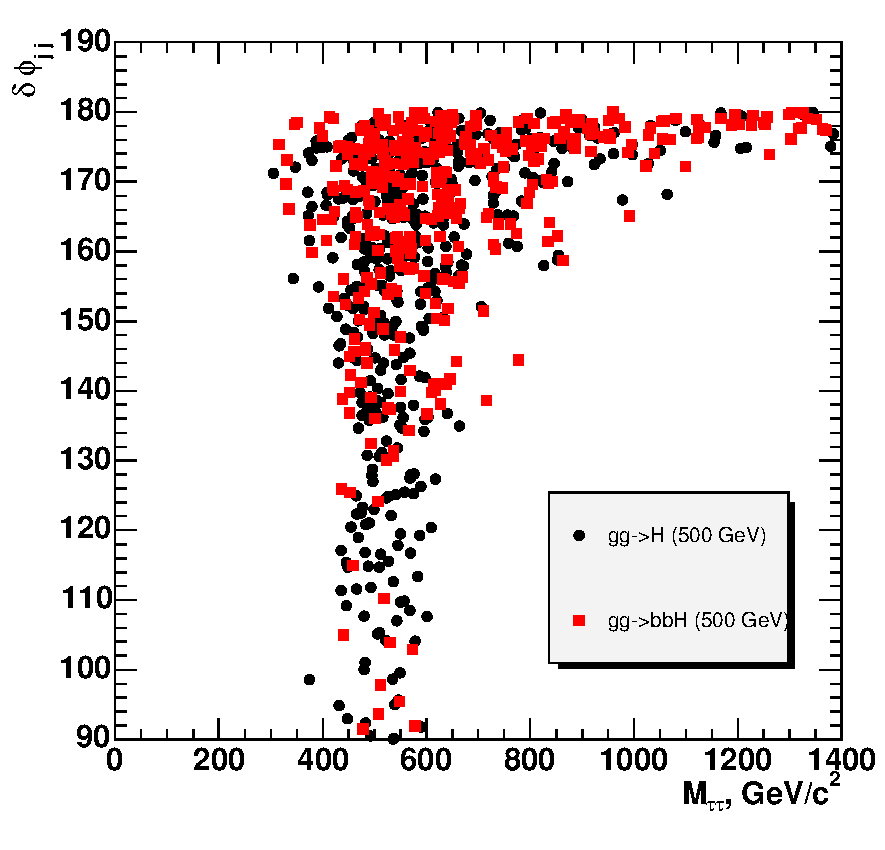
\includegraphics[width=0.45\textwidth]{analysis/mTauTau_vs_dphiJetJet_scatter_signal}
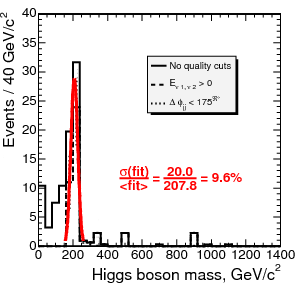
\includegraphics[width=0.45\textwidth]{analysis/HiggsMass_noQuality_200}
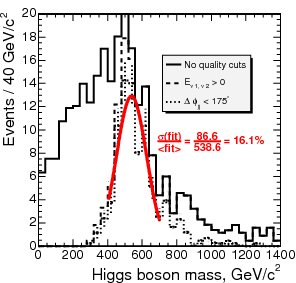
\includegraphics[width=0.45\textwidth]{analysis/HiggsMass_noQuality_500}
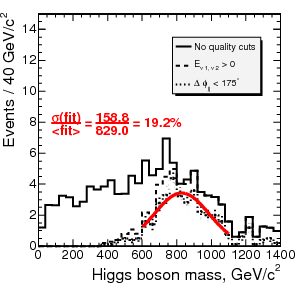
\includegraphics[width=0.45\textwidth]{analysis/HiggsMass_noQuality_800}
\caption{$M_{\tau \tau}$ scatter plot (top left) and distribution for $m_{A}$ = 200 (top right), 500 (bottom left) and 800 (bottom right)\GeVcc . The scatter plot is shown before the $\Delta \phi_{jj}$ cut. The distributions show $\mathrm{M_{\tau \tau}}$ before and after the quality cuts. The mass distribution with the $\Delta \phi$ cut has been fitted with a gaussian within the mass window ranges listed in 8.4.3.\label{fig:mass_resolution}}
\end{figure}

A mass window was formed around each $\mathrm{M_{\tau \tau}}$ peak and the number of signal and background events contained within used to calculate the discovery significance. The windows used were 150--250, 400--700 and 600--1100\GeVcc for $m_{A}$ = 200,\,500 and 800\,\GeVcc. Within the mass windows these cuts resulted in mass resolutions of 9.6\%, 16.1\% and 19.2\% for $m_{A}\mathrm{=200, 500\, and\, 800 \GeVcc}$, respectively. 

\section{Cut overview}
Table~\ref{table:cuts} shows a compete list of all cuts used in this analysis. The event kinematics for the different $m_{A}$ scenarios meant that no single set of cut parameters was appropriate for all cases. Thus the cuts were optimised separately for each of the three $m_{A}$ scenarios. The point of lowest 5$\sigma$ discovery in the \plane plane was obtained for each $m_A$ value. The lower this number the greater the area in the \plane plane that could be searched. For the analysis of real data it was assumed that other searches would place limits on the allowed values of $m_{A}$, thus allowing the appropriate cuts to be used. 

Figure~\ref{fig:cut_optimisation} shows the optimisation of individual cuts for $\tan{\beta}$ reach. Cuts were not automatically set to the lowest point for every cut-$m_A$ combination due to complications introduced by the generator level selections and the need for a statistically meaningful sample of passing events. Cuts could not be set below the value used at the generator level, which imposed a lower bound on the cut. As the cuts were increased the amount of signal and background events passing all cuts sharply decreased. Thus the seemingly lowest $\tan{\beta}$ reach could not be relied on as it may not provide a statistically meaningful result. At least 20 events were required to pass in each dataset to allow statistically meaningful conclusions to be drawn. The final cut values taken were the lowest points in Figure~\ref{fig:cut_optimisation} that were greater than the generator level selection whilst still statistically meaningful. 

%The cuts were varied as long as a significant number of events passed all cuts. This was to ensure the results were statistically meaningful. The reach was set to infinity if less than 20 signal events passed all cuts. Note that cuts were not automatically tuned to the lowest point if the background samples did not have a statistically meaningful number of events pass. 


\begin{table}[tb]
\begin{tabular}{|l|c|c|c|}
\hline
	& $m_{A}$ = 200 \GeVcc & $m_{A}$ = 500 \GeVcc & $m_{A}$ = 800 \GeVcc\\ \hline
% 	   & tan($\beta$)=20 &  tan($\beta$)=20 & tan($\beta$)=20 \\ \hline
%	\multicolumn{4}{c}{Trigger selections} \\ \hline
	Level-1 $\tau$ trigger & \multicolumn{3}{|c|}{single $\tau$ \ET = 93 GeV or Double $\tau$ \ET = 66 \GeV} \\ \hline
	HLT CaloPxl & \multicolumn{3}{|c|}{$\mathrm{P_{isol}^{cut}} = 5 \GeV, \mathrm{p_{T}^{ltr}} > 3 \GeVc, \mathrm{R_{m}} = 0.1, \mathrm{R_{S}} = 0.07, \mathrm{R_{i}}=0.5$} \\ \hline
%	\multicolumn{4}{c}{Offline selections} \\ \hline
	2 calorimeter jets &  \multicolumn{3}{|c|}{ $\ET > 10 \GeVcc$} \\ \hline
	\ET cut & 65 and 50\GeV & 100 and 50\GeV & 130 and 50\GeV \\ \hline
	2 offline $\tau$ candidates & \multicolumn{3}{|c|}{$\mathrm{R_{m} = 0.1, p_{T}^{ltr} > 10 \GeV}$} \\ \hline
	Lead track & \multicolumn{3}{|c|}{$\mathrm{p_{T}^{ltr} > 32 \GeV}$} \\ \hline
	Tracker isolation & \multicolumn{3}{|c|}{$\mathrm{R_{i}}=0.5$} \\ \hline
	Signal tracks & \multicolumn{3}{|c|}{1 track within cone $\mathrm{R_{S}} = 0.04$} \\ \hline
	$e^{-}$ rejection & \multicolumn{3}{|c|}{Hottest HCAL tower $>$ 1.5 \GeV} \\ \hline
	Charge correlation & \multicolumn{3}{|c|}{$Q_{\tau_{1}} \times Q_{\tau_{1}} = -1$} \\ \hline
	\MET & $\MET > 50 \GeV$ & $\MET > 70 \GeV$ & $\MET > 70 \GeV$ \\ \hline
%	\multicolumn{4}{c}{$M_{\tau \tau}$ quality selections} \\ \hline
	Positive energy $\nu$ & \multicolumn{3}{|c|}{$\mathrm{E_{\nu 1}, E_{\nu 2} > 0}$} \\ \hline
	Non-back-to-back jets & \multicolumn{3}{|c|}{$\mathrm{\phi_{ j j} < 175\de}$} \\ \hline
	Mass window & 150--250 \GeVcc & 400--700 \GeVcc & 600--1100 \GeVcc \\ \hline
\end{tabular}
\caption{Summary of cuts for each $m_{A}$ scenario.\label{table:cuts}}
\end{table}

\begin{figure}[tb]
\centering
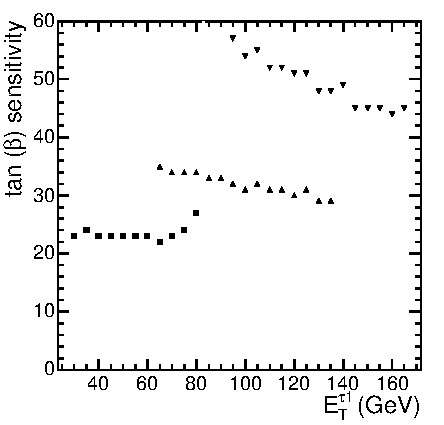
\includegraphics[width=0.45\textwidth]{analysis/OfflineJetEtCut1}
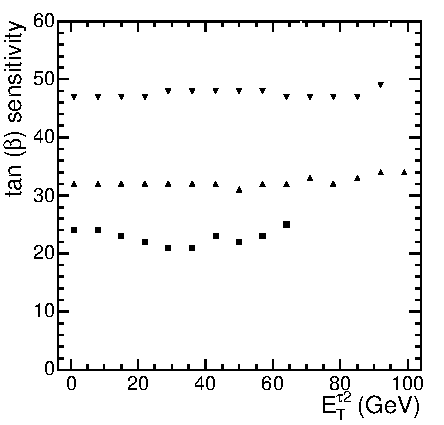
\includegraphics[width=0.45\textwidth]{analysis/OfflineJetEtCut2}
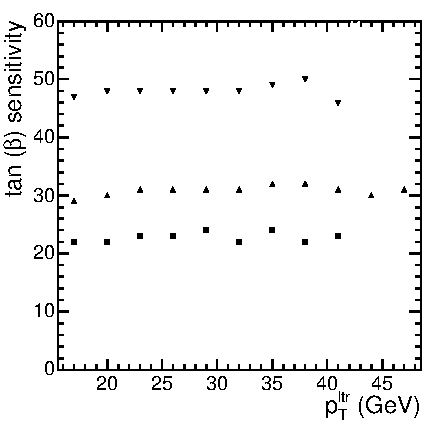
\includegraphics[width=0.45\textwidth]{analysis/OfflineleadTrackPtCut}
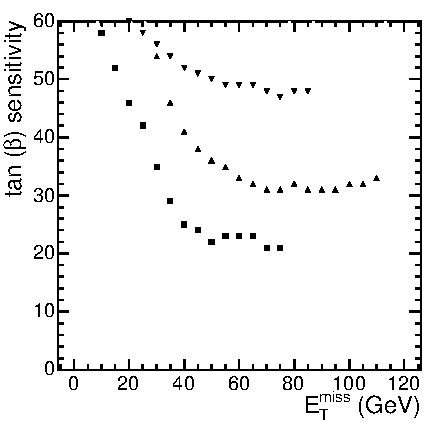
\includegraphics[width=0.45\textwidth]{analysis/OfflineMETcut}
\caption{$\tan{\beta}$ reach as a function of cut parameters. Varied cuts are \ET of most energetic $\tau$ ($\mathrm{E_{T}^{\tau 1}}$), \ET of least energetic $\tau$ ($\mathrm{E_{T}^{\tau 1}}$), \PT of $\tau$ lead track ($\mathrm{p_{T}^{ltr}}$) and \MET. Each cut is varied for 3 mass scenarios $m_A$ = 200 (squares), 500 (upward pointing triangles) and 800 (downward pointing triangles)\GeVcc.\label{fig:cut_optimisation}}
\end{figure}

\section{Efficiencies and number of events}
To obtain estimates for the expected number of events a set of MSSM parameters had to be chosen. The \mhmax scenario was used with the paramaters $M_{t} = 175\GeVcc, M_{2} = 200\GeVcc, \mu = 200 \GeVcc, X_{\rm t} = 2000\TeVcc, M_{susy} = 1\TeVcc$. These parameters are suggested in Ref~\cite{citeulike:894146}. These were used with the FeynHiggs~\cite{citeulike:905609} program to obtain cross-sections. Values of $\tan{\beta}$ were set to be close to the expected 5$\sigma$ discovery significance for 60\fb of data for each of the three $m_A$ scenarios. The actual 5$\sigma$ discovery significance is calculated later. The values of $\tan{\beta}$ used were 20, 30 and 40 for $m_A$ = 200, 500 and 800 \GeVcc, respectively. 

The signal and background efficiencies for all datasets except the QCD multijets and \Zee for each $m_{A}$ scenario are shown in Tables~\ref{table:eff_200},\,\ref{table:eff_500} and \ref{table:eff_800}. It was not possible to apply sensible cuts and have a significant number of multi-jet and \Zee events pass all cuts. Thus for these samples the cuts were factorised into three groups, where the first was applied followed independently by the second and third groups. The group efficiencies were combined to form the total efficiency. The first group contained the Level-1 trigger and offline calorimeter reconstruction. The second contained the HLT and offline $\tau$ identification. The third group contained the \MET and $\mathrm{M_{\tau \tau}}$ quality cuts. Due to the low numbers of QCD events the requirement for oppositely charged jets was not enforced for these events. Previous studies~\cite{citeulike:903864} have shown that this results in a 50\% efficiency, so this value was used. Efficiencies for the factorised cuts are shown in Tables~\ref{table:eff_fact_200}, \ref{table:eff_fact_500} and \ref{table:eff_fact_800} for $m_{A} = 200, 500 \mathrm{\,and\,} 800\GeVcc$, respectively. 

\begin{figure}[!tb]
\centering
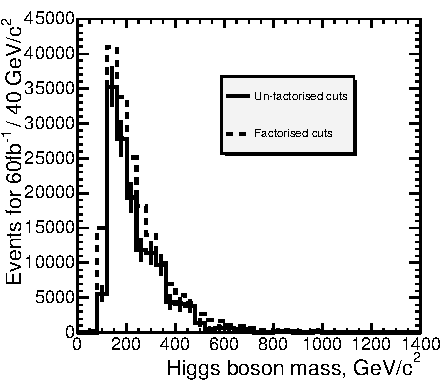
\includegraphics[width=0.45\textwidth]{analysis/Zee}
\caption{$M_{\tau \tau}$ distributions for \Zee with and without factorised cut groups. Obtained with relaxed cuts: \ET $>$ 30 \GeV, $\mathrm{p_{T}^{ltr} > 10 \GeV}$, \MET $>$ 10 \GeV and hot HCAL tower $>$ 0.5 \GeV.\label{fig:zee_factorised}}
\end{figure}

The cut factorisation was not applied to all samples as the cut groups were not independent for samples containing genuine $\tau$ jets. The $\mathrm{M_{\tau \tau}}$ distribution obtained with relaxed cuts for \Zee, with and without factorised cut groups, is shown in Figure~\ref{fig:zee_factorised}. The two distributions were compared with the Kolmogorov test and a similarity of 27.8\% obtained. It can be seen that the factorised cuts resulted in an over-estimation of the distribution. As the factorisation was only applied to background datasets this resulted in a higher background than would otherwise be expected. Thus results obtained represented a worst case scenario. A comparison of the multi-jets was not performed as not enough Monte Carlo events passed all cuts even when they were relaxed.

Some data samples that had been generated in multiple \ET/mass ranges had no events in a set range that passed all cuts. This was because they fell outside of the signal region, i.e. their generated \ET was below the cut or their invariant mass was outside the mass window.

The \TopTop, \Wjet\,and some QCD multi-jet datasets ran out of events before passing all selections in certain $m_{A}$ scenarios. Factorised cuts could not be used for the \Wjet\xspace or \TopTop\xspace  samples as they contained genuine $\tau$ jets. In these cases the cuts were loosened until a significant number of Monte Carlo events passed. These were then used to obtain a prediction for the upper bound on the expected number of background events.

\begin{figure}[!Hhtb]
\centering
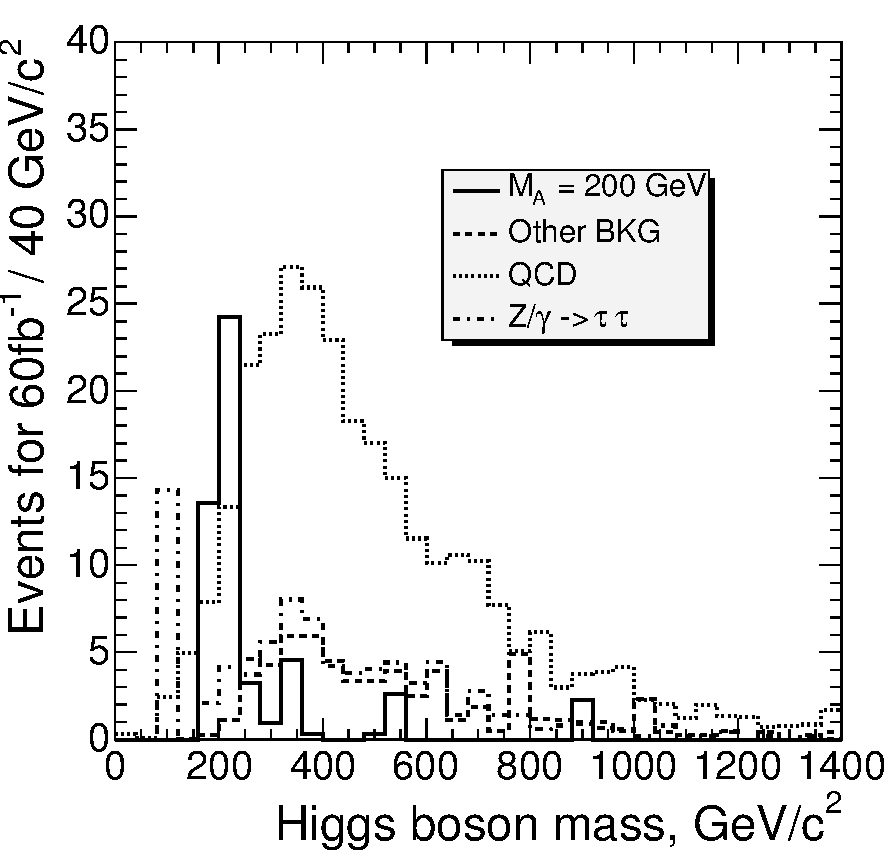
\includegraphics[width=0.45\textwidth]{analysis/HiggsMass_200}
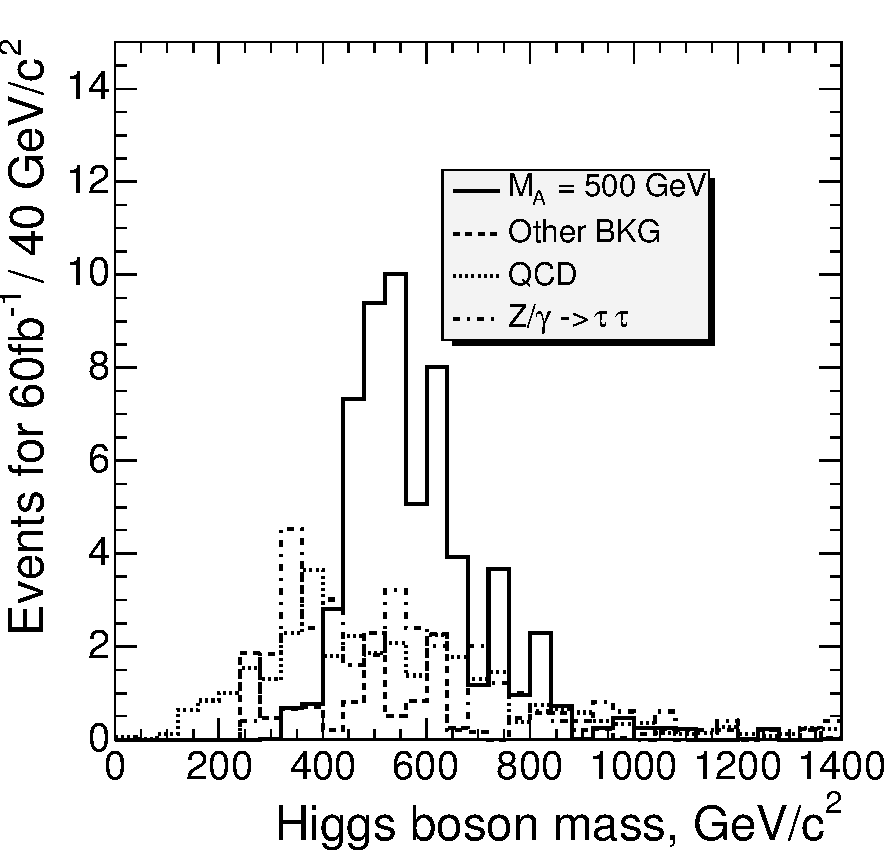
\includegraphics[width=0.45\textwidth]{analysis/HiggsMass_500}
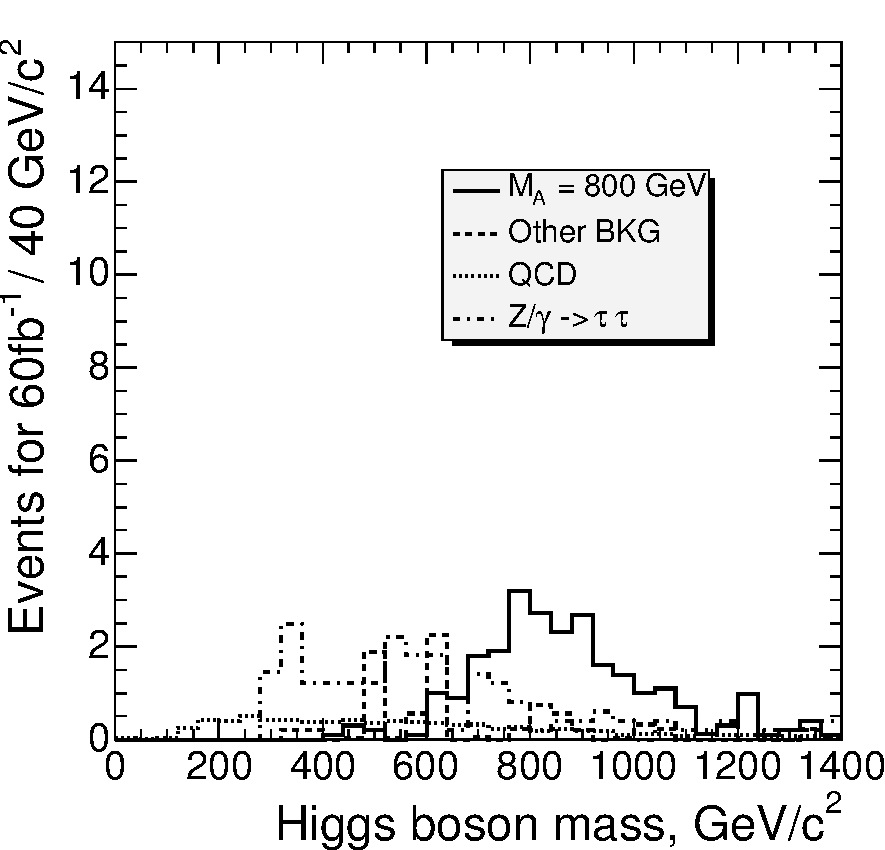
\includegraphics[width=0.45\textwidth]{analysis/HiggsMass_800}
\caption{$M_{\tau \tau}$ distributions for expected signal and background for $m_{A} = 200,\,500\, \mathrm{and}\,800\GeVcc$ in the \mhmax scenario with $\tan{\beta}$ = 20, 30 and 40 scaled for 60 \fb of data.\label{fig:mass_plots}}
\end{figure}

\begin{sidewaystable}
	\centering
	  \begin{tabular}{|l|c|c|c|c|c|c|c|c|}
  \hline
& $ \bbH $
& $ \ggH $
& $ \TopTop $
& $ \Wjet $
& $ \Wtb $
& $ \ZTauTau$
& $ \ZTauTau$
& $ \ZTauTau$
\\
& & & & &  & \ZTauTaua & \ZTauTaub & \ZTauTauc
\\ \hline
$\sigma \times BR \times \epsilon_{kine}$ & 3753 & 476 & 281 & 12398 & 9.8 & 29830 & 1182 & 201 \\ \hline
L1 $\tau$ Trigger & 0.501 & 0.519 & 0.753 & 0.784 & 0.826 & 0.530 & 0.702 & 0.859 \\ \hline
HLT CaloPxl & 0.291 & 0.246 & 0.047 & 0.034 & 0.128 & 0.046 & 0.192 & 0.241 \\ \hline
2 offline calorimeter $\tau$ jets & 0.997 & 0.998 & 0.994 & 0.995 & 0.997 & 0.984 & 0.999 & 0.999 \\ \hline
$\tau E_{T}^{cut}$ & 0.347 & 0.348 & 0.562 & 0.725 & 0.585 & 0.241 & 0.415 & 0.842 \\ \hline
2 offline $\tau$ candidates & 0.678 & 0.688 & 0.815 & 0.800 & 0.795 & 0.693 & 0.699 & 0.713 \\ \hline
$\mathrm{p_{T}^{ltr}}$ cut & 0.404 & 0.403 & 0.661 & 0.639 & 0.749 & 0.290 & 0.410 & 0.600 \\ \hline
Tracker isolation & 0.855 & 0.854 & 0.825 & 0.476 & 0.852 & 0.638 & 0.850 & 0.918 \\ \hline
Signal tracks & 0.592 & 0.587 & 0.567 & 0.254 & 0.544 & 0.378 & 0.580 & 0.643 \\ \hline
Hottest HCAL Tower & 0.954 & 0.989 & 0.903 & 0.965 & 0.921 & 0.941 & 0.904 & 0.877 \\ \hline
$\mathrm{Q_{\tau 1} x Q_{\tau 2}}$ = -1 & 0.979 & 0.962 & 0.958 & 0.835 & 0.940 & 0.594 & 0.950 & 0.943 \\ \hline
\MET & 0.088 & 0.128 & 0.607 & 0.295 & 0.472 & 0.158 & 0.129 & 0.443 \\ \hline
$\mathrm{E_{\nu 1}, E_{\nu 2}} >$ 0 & 0.298 & 0.507 & 0.426 & 0.138 & 0.383 & 0.333 & 0.475 & 0.470 \\ \hline
$\mathrm{\phi_{j j} < 175\de}$ & 0.824 & 0.882 & 0.867 & 0.467 & 0.861 & 1.000 & 0.679 & 0.502 \\ \hline
Mass window efficiencies&  1.21 \ten{-4}  & 2.77 \ten{-4} &  0.000  &  0.000  &  6.67 \ten{-5} &  0.000  &  5.9 \ten{-5} &  0.000  \\ \hline
Mass window $\sigma (\fbplus)$ &  0.454  &  0.133  &  0.000  &  0.000  &  6.53\ten{-4} &  0.000  &  0.0695  &  0.000  \\ \hline
expected events for 60 $(\fb)$ &  27.3  &  7.94  &  0.000  &  0.000  &  0.0391  &  0.000  &  4.17  &  0.000  \\ \hline
\end{tabular}

	\caption{Efficiencies for signal and background events in the $m_{A} = 200 \GeV$ scenario. $\mathrm{M_{Z}}$ in \GeVcc\label{table:eff_200}}
\end{sidewaystable}

\begin{sidewaystable}
	\centering
	  \begin{tabular}{|l|c|c|c|c|c|}
  \hline
& $ \QCD$
& $ \QCD$
& $ \QCD$
& $ \QCD$
& $ \Zee $
\\
& $ 50 < \pthat < 80\GeV$ & $80 < \pthat < 120\GeV$ & $120 < \pthat < 170\GeV$ & $\pthat > 170\GeV$ &
\\ \hline
$\sigma \times BR \times \epsilon_{kine}$ & 5.08 \ten{6} & 1.70 \ten{7} & 2.11 \ten{7} & 2.82 \ten{7} & 3.97 \ten{6} \\ \hline
L1 $\tau$ Trigger & 0.461 & 0.716 & 0.727 & 0.562 & 0.106 \\ \hline
2 offline calorimeter $\tau$ jets & 0.995 & 0.982 & 0.976 & 0.976 & 0.995 \\ \hline
$\tau E_{T}^{cut}$ & 0.121 & 0.665 & 0.784 & 0.742 & 0.060 \\ \hline
Group 1 cuts &  0.0551 &  0.462  &  0.544  &  0.393  &  0.00622  \\ \hline
HLT CaloPxl & 0.012 & 0.005 & 0.002 & 0.001 & 0.133 \\ \hline
2 offline $\tau$ candidates & 0.879 & 0.839 & 0.860 & 0.830 & 0.554 \\ \hline
$\mathrm{p_{T}^{ltr}}$ cut & 0.608 & 0.647 & 0.569 & 0.547 & 0.741 \\ \hline
Tracker isolation & 0.323 & 0.244 & 0.264 & 0.216 & 0.907 \\ \hline
Signal tracks & 0.100 & 0.216 & 0.250 & 0.067 & 0.937 \\ \hline
Hottest HCAL Tower & 1.000 & 1.000 & 1.000 & 1.000 & 0.007 \\ \hline
$\mathrm{Q_{\tau 1} x Q_{\tau 2}}$ = -1 & 0.500 & 0.500 & 0.500 & 0.500 & 1.00 \\ \hline
Group 2 cuts &  2.00\ten{-3} &  1.32\ten{-3} & 5.75 \ten{-5} & 5.21 \ten{6} &  3.26\ten{-3}  \\ \hline
\MET & 0.006 & 0.008 & 0.024 & 0.086 & 0.047 \\ \hline
$\mathrm{E_{\nu 1}, E_{\nu 2}} >$ 0 & 0.448 & 0.474 & 0.430 & 0.482 & 0.502 \\ \hline
$\mathrm{\phi_{j j} < 175\de}$ & 0.462 & 0.720 & 0.684 & 0.741 & 0.842 \\ \hline
Group 3 cuts &  0.00120  &  0.00264  &  0.00712  &  0.0308  &  0.0201  \\ \hline
Mass window efficiencies &  0.000  &  7.75 \ten{-9}  &  8.26 \ten{-9}  & 3.34 \ten{-9}  &  1.99 \ten{-9}  \\ \hline
Mass window $\sigma (\fbplus)$ &  0.000  &  0.132  &  0.174  &  0.0943  &  0.00789  \\ \hline
expected events for 60 $(\fb)$ &  0.000  &  7.89  &  10.4  &  5.66  &  0.473  \\ \hline
\end{tabular}

	\caption{Efficiencies for factorised background events in the $m_{A} = 200 \GeV$ scenario\label{table:eff_fact_200}}
\end{sidewaystable}

\begin{sidewaystable}
	\centering
	  \begin{tabular}{|l|c|c|c|c|c|c|c|c|}
  \hline
& $ \bbH $
& $ \ggH $
& $ \TopTop $
& $ \Wjet $
& $ \Wtb $
& $ \ZTauTau$
& $ \ZTauTau$
& $ \ZTauTau$
\\
& & & & &  & \ZTauTaua & \ZTauTaub & \ZTauTauc
\\ \hline
$\sigma \times BR \times \epsilon_{kine}$ & 186 & 6.31 & 281 & 12398 & 9.80 & 29830 & 1181 & 201 \\ \hline
L1 $\tau$ Trigger & 0.853 & 0.858 & 0.753 & 0.784 & 0.826 & 0.530 & 0.702 & 0.859 \\ \hline
HLT CaloPxl & 0.322 & 0.267 & 0.047 & 0.034 & 0.128 & 0.046 & 0.192 & 0.241 \\ \hline
2 offline calorimeter $\tau$ jets & 0.999 & 0.999 & 0.994 & 0.995 & 0.997 & 0.984 & 0.999 & 0.999 \\ \hline
$\tau E_{T}^{cut}$ & 0.756 & 0.753 & 0.270 & 0.349 & 0.287 & 0.073 & 0.097 & 0.639 \\ \hline
2 offline $\tau$ candidates & 0.717 & 0.710 & 0.816 & 0.812 & 0.778 & 0.737 & 0.725 & 0.717 \\ \hline
$\mathrm{p_{T}^{ltr}}$ cut & 0.662 & 0.659 & 0.671 & 0.667 & 0.776 & 0.459 & 0.505 & 0.634 \\ \hline
Tracker isolation & 0.950 & 0.942 & 0.845 & 0.486 & 0.852 & 0.583 & 0.840 & 0.922 \\ \hline
Signal tracks & 0.671 & 0.662 & 0.570 & 0.211 & 0.538 & 0.286 & 0.562 & 0.653 \\ \hline
Hottest HCAL Tower & 0.984 & 0.976 & 0.904 & 0.945 & 0.927 & 1.000 & 0.902 & 0.881 \\ \hline
$\mathrm{Q_{\tau 1} x Q_{\tau 2}}$ = -1 & 0.937 & 0.947 & 0.935 & 0.824 & 0.922 & 0.583 & 0.942 & 0.941 \\ \hline
\MET & 0.385 & 0.436 & 0.462 & 0.290 & 0.406 & 0.143 & 0.115 & 0.327 \\ \hline
$\mathrm{E_{\nu 1}, E_{\nu 2}} >$ 0 & 0.428 & 0.529 & 0.452 & 0.133 & 0.372 & 0.000 & 0.333 & 0.477 \\ \hline
$\mathrm{\phi_{j j} < 175\de}$ & 0.523 & 0.753 & 0.848 & 0.500 & 0.812 & 0.000 & 0.800 & 0.527 \\ \hline
Mass window efficiencies&  0.004  &  6.76\ten{-4}  &  1.15\ten{-4} &  5.04\ten {-6} &  5.33\ten{-4} &  0.000  &  0.000  &  0.00125  \\ \hline
Mass window $\sigma (\fbplus)$ &  0.745  &  0.0426  &  0.0324  &  0.0625  &  0.00523  &  0.000  &  0.000  &  0.252  \\ \hline
expected events for 60 $(\fb)$ &  44.7  &  2.56  &  1.95  &  3.75  &  0.313  &  0.000  &  0.000  & 15.1  \\ \hline
\end{tabular}

	\caption{Efficiencies for signal and background events in the $m_{A} = 500 \GeV$ scenario. $\mathrm{M_{Z}}$ in \GeVcc\label{table:eff_500}}
\end{sidewaystable}

\begin{sidewaystable}
	\centering
	  \begin{tabular}{|l|c|c|c|c|c|}
  \hline
& $ \QCD$
& $ \QCD$
& $ \QCD$
& $ \QCD$
& $ \Zee$
\\
& $ 50 < \pthat < 80\GeV$ & $80 < \pthat < 120\GeV$ & $120 < \pthat < 170\GeV$ & $\pthat > 170\GeV$ &
\\ \hline
$\sigma \times BR \times \epsilon_{kine}$ & 5.08 \ten{6} & 1.70 \ten{7} & 2.11 \ten{7} & 2.82 \ten{7} & 3.97 \ten{6} \\ \hline
L1 $\tau$ Trigger & 0.461 & 0.716 & 0.727 & 0.562 & 0.106 \\ \hline
2 offline calorimeter $\tau$ jets & 0.995 & 0.982 & 0.976 & 0.976 & 0.995 \\ \hline
$\tau E_{T}^{cut}$ & 0.001 & 0.061 & 0.467 & 0.667 & 0.020 \\ \hline
Group 1 cuts &  4.61\ten{-4} & 0.0421  &  0.324  &  0.354  &  0.00205  \\ \hline
HLT CaloPxl & 0.024 & 0.004 & 0.002 & 0.001 & 0.112 \\ \hline
2 offline $\tau$ candidates & 1.000 & 0.903 & 0.848 & 0.838 & 0.623 \\ \hline
$\mathrm{p_{T}^{ltr}}$ cut & 0.000 & 0.679 & 0.571 & 0.564 & 0.768 \\ \hline
Tracker isolation & 0.000 & 0.158 & 0.234 & 0.195 & 0.890 \\ \hline
Signal tracks & 0.000 & 0.667 & 0.200 & 0.040 & 0.897 \\ \hline
Hottest HCAL Tower & 0.000 & 1.000 & 1.000 & 1.000 & 0.011 \\ \hline
$\mathrm{Q_{\tau 1} x Q_{\tau 2}}$ = -1 & 0.000 & 0.500 & 0.500 & 0.500 & 1.00 \\ \hline
Group 2 cuts &  0.000  &  2.65\ten{-4} &  4.83 \ten{-5} &  2.90 \ten{-6}  & 4.93\ten{-3} \\ \hline
\MET & 0.024 & 0.001 & 0.004 & 0.034 & 0.022 \\ \hline
$\mathrm{E_{\nu 1}, E_{\nu 2}} >$ 0 & 1.000 & 0.556 & 0.535 & 0.555 & 0.523 \\ \hline
$\mathrm{\phi_{j j} < 175\de}$ & 0.000 & 0.800 & 0.809 & 0.819 & 0.783 \\ \hline
Group 3 cuts &  0.000  &  5.29\ten{-4} &  0.00177  &  0.0155  &  0.00888  \\ \hline
Mass window efficiencies &  0.000  &  7.37 \ten{-10}  &  6.81 \ten{-9}  &  2.61 \ten{-9}  &  5.01 \ten{-9}  \\ \hline
Mass window $\sigma (\fbplus)$ &  0.000  &  0.0125  &  0.144  &  0.0736  &  0.0199  \\ \hline
expected events for 60 $(\fb)$ &  0.000  &  0.750  &  8.61  &  4.42  &  1.19  \\ \hline
\end{tabular}

	\caption{Efficiencies for factorised background events in the $m_{A} = 500 \GeV$ scenario\label{table:eff_fact_500}}
\end{sidewaystable}

\begin{sidewaystable}
	\centering
	  \begin{tabular}{|l|c|c|c|c|c|c|c|c|}
  \hline
& $ \bbH$
& $ \ggH$
& $ \TopTop$
& $ \Wjet$
& $ \Wtb$
& $ \ZTauTau$
& $ \ZTauTau$
& $ \ZTauTau$
\\
& & & & &  &\ZTauTaua&\ZTauTaub&\ZTauTauc\\ \hline
$\sigma \times BR \times \epsilon_{kine}$ & 49 & 0.722 & 281 & 12398 & 9.80 & 29830 & 1181 & 200 \\ \hline
L1 $\tau$ Trigger & 0.896 & 0.875 & 0.753 & 0.784 & 0.826 & 0.530 & 0.702 & 0.859 \\ \hline
HLT CaloPxl & 0.316 & 0.247 & 0.047 & 0.034 & 0.128 & 0.046 & 0.192 & 0.241 \\ \hline
2 offline calorimeter $\tau$ jets & 1.000 & 0.999 & 0.994 & 0.995 & 0.997 & 0.984 & 0.999 & 0.999 \\ \hline
$\tau E_{T}^{cut}$ & 0.832 & 0.782 & 0.121 & 0.170 & 0.132 & 0.027 & 0.019 & 0.411 \\ \hline
2 offline $\tau$ candidates & 0.679 & 0.679 & 0.796 & 0.813 & 0.787 & 0.722 & 0.762 & 0.720 \\ \hline
$\mathrm{p_{T}^{ltr}}$ cut & 0.746 & 0.743 & 0.688 & 0.694 & 0.782 & 0.421 & 0.557 & 0.663 \\ \hline
Tracker isolation & 0.951 & 0.948 & 0.845 & 0.500 & 0.858 & 0.667 & 0.795 & 0.930 \\ \hline
Signal tracks & 0.785 & 0.774 & 0.653 & 0.185 & 0.661 & 0.062 & 0.586 & 0.675 \\ \hline
Hottest HCAL Tower & 0.983 & 0.984 & 0.948 & 0.967 & 0.917 & 1.000 & 0.882 & 0.874 \\ \hline
$\mathrm{Q_{\tau 1} x Q_{\tau 2}}$ = -1 & 0.936 & 0.941 & 0.945 & 0.795 & 0.924 & 0.000 & 0.900 & 0.940 \\ \hline
\MET & 0.568 & 0.601 & 0.477 & 0.543 & 0.475 & 0.000 & 0.407 & 0.400 \\ \hline
$\mathrm{E_{\nu 1}, E_{\nu 2}} >$ 0 & 0.468 & 0.553 & 0.366 & 0.132 & 0.328 & 0.000 & 0.364 & 0.450 \\ \hline
$\mathrm{\phi_{j j} < 175\de}$ & 0.452 & 0.664 & 0.800 & 0.400 & 0.789 & 0.000 & 0.750 & 0.498 \\ \hline
Mass window efficiencies &  0.00827 &  0.0108 &  8.97\ten{-5} &  2.52\ten{-6} & 2.66\ten{-4} &  0.000 &  0.000 &  7.00\ten{-4} \\ \hline
Mass window $\sigma (\fbplus)$ &  0.405 &  0.00783 &  0.0252 &  0.0312 &  0.00261 &  0.000 &  0.000 &  0.141 \\ \hline
expected events for 60 (\fb) &  24.3 &  0.470 &  1.51 &  1.87 &  0.157 &  0.000 &  0.000 &  8.44 \\ \hline
\end{tabular}

	\caption{Efficiencies for signal and background events in the $m_{A} = 800 \GeV$ scenario. $\mathrm{M_{Z}}$ in \GeVcc\label{table:eff_800}}
\end{sidewaystable}

\begin{sidewaystable}
	\centering
	  \begin{tabular}{|l|c|c|c|c|c|}
  \hline
& $ \QCD$
& $ \QCD$
& $ \QCD$
& $ \QCD$
& $ \Zee $
\\
& $ 50 < \pthat < 80\GeV$ & $80 < \pthat < 120\GeV$ & $120 < \pthat < 170\GeV$ & $\pthat > 170\GeV$ &
\\ \hline
$\sigma \times BR \times \epsilon_{kine}$ & 5.08 \ten{6} & 1.70 \ten{7} & 2.11 \ten{7} & 2.82 \ten{7} & 3.97 \ten{6} \\ \hline
L1 $\tau$ Trigger & 0.461 & 0.716 & 0.727 & 0.562 & 0.106 \\ \hline
2 offline calorimeter $\tau$ jets & 0.995 & 0.982 & 0.976 & 0.976 & 0.995 \\ \hline
$\tau E_{T}^{cut}$ &  9.68 \ten{-5}  & 0.003 & 0.099 & 0.536 & 0.007 \\ \hline
Group 1 cuts &  4.39 \ten{-5}  &  0.00231  &  0.0689  &  0.285  &  0.000765  \\ \hline
HLT CaloPxl & 0.000 & 0.007 & 0.002 & 0.001 & 0.101 \\ \hline
2 offline $\tau$ candidates & 0.000 & 0.667 & 0.862 & 0.811 & 0.618 \\ \hline
$\mathrm{p_{T}^{ltr}}$ cut & 0.000 & 0.500 & 0.640 & 0.574 & 0.872 \\ \hline
Tracker isolation & 0.000 & 0.000 & 0.125 & 0.218 & 0.902 \\ \hline
Signal tracks & 0.000 & 0.000 & 0.000 & 0.045 & 0.865 \\ \hline
Hottest HCAL Tower & 0.000 & 0.000 & 0.000 & 1.000 & 0.031 \\ \hline
$\mathrm{Q_{\tau 1} x Q_{\tau 2}}$ = -1 & 0.000 & 0.500 & 0.500 & 0.500 & 1.00 \\ \hline
Group 2 cuts &  0.000  &  0.000  &  0.000  &  3.61 \ten{-6}  &  0.00133  \\ \hline
\MET & 0.000 & 0.000 & 0.008 & 0.033 & 0.038 \\ \hline
$\mathrm{E_{\nu 1}, E_{\nu 2}} >$ 0 & 0.000 & 0.000 & 0.535 & 0.542 & 0.483 \\ \hline
$\mathrm{\phi_{j j} < 175\de}$ & 0.000 & 0.000 & 0.759 & 0.786 & 0.714 \\ \hline
Group3 cuts &  0.000  &  0.000  &  0.00311  &  0.0139  &  0.0133  \\ \hline
Mass window efficiencies &  0.000 &  0.000 & 0.000 &  2.35 \ten{-9} &  6.73 \ten{-9} \\ \hline
Mass window $\sigma (\fbplus)$ & 0.000 &  0.000 &  0.000 &  0.0661 &  0.0267 \\ \hline
expected events for 60 (\fb) &  0.000 &  0.000 &  0.000 &  3.97 &  1.60 \\ \hline
\end{tabular}

	\caption{Efficiencies for factorised background events in the $m_{A} = 800 \GeV$ scenario\label{table:eff_fact_800}}
\end{sidewaystable}

Figure~\ref{fig:mass_plots} shows the $\mathrm{M}_{\tau \tau}$ plots for all $m_{A}$ scenarios. The expected number of signal and background events and the discovery significance can be seen in Table~\ref{table:events}. It can be seen that the major background processes were QCD multi-jets and \Ztautau.

\begin{table}[!Hhtb]
	\centering
\begin{tabular}{|l|c|c|c|}
\hline
process & \multicolumn{3}{|c|}{$m_{A}$ (\GeVcc)} \\ \hline
 & 200  & 500 & 800\\ \hline
\bbH & 27.3 & 44.7 & 24.3\\ \hline
\ggH & 7.9 & 2.6 & 0.47\\ \hline
QCD multijets & $< 25.6$  & 13.8 & $< 6.7$\\ \hline
\Ztautau & 4.2 & 15.1 & 8.4\\ \hline
\Zee & 0.5 & 1.2 & 1.6\\ \hline
\TopTop  & $< 0.43$ & 1.9 & 1.5\\ \hline
\Wjet & $< 1.87$ & 3.7 & 1.9\\ \hline
\Wtb & 0.04 & 0.31 & 0.16\\ \hline
$S/\sqrt{B}$ & 6.2 & 7.8 & 5.5 \\ \hline
\end{tabular}
\caption{Summary of expected events for all 3 mass scenarios for 60\fb in the \mhmax scenario.\label{table:events}}
\end{table}

\section{Evaluation of background from data and systematics}
The background uncertainty was calculated for the two main backgrounds, QCD multi-jets and \Ztautau. 

\subsection{QCD multi-jets}
The QCD multi-jet background could be directly measured from the data by replacing the requirement for jets of opposite electric charge with one for same sign jets. This requirement effectively suppressed all other signal and backgrounds. The number of same sign and opposite sign QCD multi-jet events was equal so a direct measurement of the uncertainty on the number of events was possible. Expected number of events was calculated with all cuts except the mass window. The expected events were 296.5, 34.0, and 8.6 for $m_{A}$ = 200, 500 and 800\GeVcc respectively, giving uncertainties of 5.8, 17.2 and 34.2\%.

\subsection{\Ztautau}
It was not possible to isolate the \Ztautau\xspace background hence the uncertainty on the number of events had to be computed. The total uncertainty, $\mathrm{\Delta_{Z_{\tau \tau}}}$, could be computed:

\begin{equation}
	\mathrm{\Delta_{Z_{\tau \tau}}} = \Delta_{theory} \oplus \Delta_{L} \oplus \Delta_{\epsilon}
\end{equation}

with the terms on the right-hand side representing the uncertainties on the theory (cross section and branching ratio), LHC luminosity and experimental efficiency, respectively. The uncertainty on the $\mathrm{Z \rightarrow \tau \tau}$ branching ratio was small ($\simeq$ 0.1\%) and hence neglected~\cite{pdg2006}. $\Delta_{theory} = 3\%$ was taken from the uncertainty on the cross section~\cite{citeulike:891490}. The nominal CMS value for $\Delta_{L}$ was 3\% for 30 \fb of data and above~\cite{CMS_TDR_PHYS_vol2}.

The experimental selection uncertainty could be computed:

\begin{equation}
	\Delta_{\epsilon} = \Delta_{jet\,scale} \oplus \Delta_{MET} \oplus \Delta_{\tau\,tagging}
\end{equation}

where the energy terms on the right-hand side represent the uncertainty of the experimental selection due to the jet scale, \MET scale and $\tau$ tagging, respectively. The $\tau$ tagging efficiency was calculated as 8.8\% for each $\tau$~\cite{citeulike:905602}. 

\subsubsection{Jet scale}
CMS has calculated that, with 30\,\fb of data or more, the CMS jet scale uncertainty will be 3\% and the calorimeter scale 10\%~\cite{CMS_TDR_PHYS_vol2}. No study of the $\tau$ jet scale systematics had been performed to date so the standard jet uncertainty was used for both $\tau$ and multi-jets. The effect of the jet scale uncertainty is shown in Table~\ref{tab:jetScale}.

\begin{table}[!Hh]
	\centering
	\begin{tabular}{|c|c|c|c|c|c|}
	\hline
	$m_{A}$ scenario & $\epsilon_{0}$ & $\epsilon_{-}$ & $\epsilon_{+}$ & $\epsilon_{+} - \epsilon_{-}$ & \% variation\\ \hline
	200\GeVcc & 0.000324 & 0.000309 & 0.000353 & 0.0000221 & 6.18\\ \hline
	500\GeVcc & 0.00245 & 0.00233 & 0.00258 & 0.000125 & 5.10\\ \hline
	800\GeVcc & 0.00167 & 0.00155 & 0.00178 & 0.000117 & 7.00\\ \hline
    \end{tabular}
\caption{$\Ztautau$ efficiency for 3 different jet scale scenarios. Scenarios are nominal jet scale $\epsilon_{0}$ and $\pm3\%$ ($\epsilon_{\pm}$) variation.\label{tab:jetScale}}
\end{table}

\subsubsection{\MET scale}
$\Delta_{MET}$ was calculated for the corrected \MET as shown in Equation~\ref{eqn:MET_corr}. The equation may be rewritten to separate the terms dependent on the two calorimeter scale uncertainties: 

\begin{equation}
\rm E _{\rm Tx(y)}^{miss}= -([\rm E _{Tx(y)}^{\rm raw}-
                           \sum  _{jets}\rm E _{\rm Tx(y)}^{\rm raw jet}] _{\rm low~\rm E _{\rm T}} +
                           [\sum _{jets}\rm E _{\rm Tx(y)}^{\rm corr.jet}] _{\rm high~E _{\rm T}})
\end{equation}

The calorimeter and jet scale variations were applied independently and the maximal deviations measured. Results for the various $m_{A}$ scenarios are shown in Tables~\ref{tab:metScale200}, \ref{tab:metScale500} and \ref{tab:metScale800}.

\begin{table}[!Hh]
	\centering
	\begin{tabular}{|c|c|c|c|c|}
	\hline
	Calorimeter scale variation & jet scale variation & $\epsilon$ \\ \hline
	1.0   &  1.0  &   0.000324 \\ \hline
	1.1   &  1.03 &   0.000353 \\ \hline
	1.1   &  0.97 &   0.000338 \\ \hline
	0.9   &  1.03 &   0.000309 \\ \hline
	0.9   &  0.97 &   0.000294 \\ \hline
	\multicolumn{2}{|c|}{Maximal variation} & 9.09 \% \\ \hline          
    \end{tabular}
\caption{$\Ztautau$ \MET efficiency for various calorimeter and jet scale variations in the $m_{A} = 200 \GeVcc$ scenario.\label{tab:metScale200}}
\end{table}

\begin{table}[!Hh]
	\centering
	\begin{tabular}{|c|c|c|c|c|}
	\hline
	Calorimeter scale variation & jet scale variation & $\epsilon$ \\ \hline
	1.0   &  1.0  &   0.00245 \\ \hline
	1.1   &  1.03  &  0.00272 \\ \hline
	1.1   &  0.97  &  0.00275 \\ \hline
	0.9   &  1.03  &  0.00232 \\ \hline
	0.9   &  0.97  &  0.00232 \\ \hline
	\multicolumn{2}{|c|}{Maximal range} & 8.84 \% \\ \hline          
    \end{tabular}
\caption{$\Ztautau$ \MET efficiency for various calorimeter and jet scale variations in the $m_{A} = 500 \GeVcc$ scenario.\label{tab:metScale500}}
\end{table}

\begin{table}[!Hh]
	\centering
	\begin{tabular}{|c|c|c|c|c|}
	\hline
	Calorimeter scale variation & jet scale variation & $\epsilon$ \\ \hline
	1.0   &  1.0   &  0.00167 \\ \hline
	1.1   &  1.03  &  0.00183 \\ \hline
	1.1   &  0.97  &  0.00173 \\ \hline
	0.9   &  1.03  &  0.00157 \\ \hline
	0.9   &  0.97  &  0.00153 \\ \hline
	\multicolumn{2}{|c|}{Maximal range} & 9.00 \% \\ \hline          
    \end{tabular}
\caption{$\Ztautau$ \MET efficiency for various calorimeter and jet scale variations in the $m_{A} = 800 \GeVcc$ scenario.\label{tab:metScale800}}
\end{table}
\newpage
\subsubsection{Total \Ztautau\xspace uncertainty}
The \Ztautau\,background uncertainty constituents were combined and the final values computed are shown in Table~\ref{tab:zUncertain}.

\begin{table}[!Hh]
	\centering
	\begin{tabular}{|c|c|c|c|c|c|c|}
	\hline
	$m_{A} (\GeVcc)$ & $\Delta_{theory}$ & $\Delta_{L}$ & $\Delta_{jet scale}$ & $\Delta_{MET}$ & $\Delta_{\tau tagging}$ & $\Delta_{Z_{\tau \tau}}$ \\ \hline
	200 & 0.03 & 0.03 & 0.0618 & 0.0909 & 2 $\times$ 0.088 & 0.166 \\ \hline
	500 & 0.03 & 0.03 & 0.0510 & 0.0884 & 2 $\times$ 0.088 & 0.158 \\ \hline
	800 & 0.03 & 0.03 & 0.07 & 0.09 & 2 $\times$ 0.088 & 0.166 \\ \hline 
    \end{tabular}
\caption{\Ztautau\xspace background uncertainty for $m_{A} = 200, 500 \mathrm{\,and\,} 800 \GeVcc$.\label{tab:zUncertain}}
\end{table}

\subsection{Total uncertainty}
The total background uncertainties were then formed from the QCD multi-jet and \ZTauTau uncertainties	:
\begin{equation}
	\mathrm{\Delta_{200} = 5.8 \oplus 16.6 = 17.6\%}
\end{equation}
\begin{equation}
	\mathrm{\Delta_{500} = 17.2 \oplus 15.8 = 23.4\%}
\end{equation}
\begin{equation}
	\mathrm{\Delta_{800} = 34.2 \oplus 16.6 = 38.0\%}
\end{equation}

\section{Discovery reach in \plane plane}
The 5$\sigma$ discovery significance was calculated with Poisson statistics~\cite{citeulike:905688} of the number of events within each mass window and the background uncertainties from the previous section. The reach for the three $m_{A}$ scenarios can be seen in Table~\ref{table:discovery} and Figure~\ref{fig:discovery} along with the values for the b-tagging study. 

\begin{table}[!Hhtb]
	\centering
\begin{tabular}{|l|l|c|c|c|}
\hline
%process & \multicolumn{3}{|c|}{$m_{A}$} \\ \hline
Analysis& & $m_{A} = 200\GeVcc$ & $m_{A} = 500\GeVcc$ & $M_{A} = 800\GeVcc$ \\ \hline
\cline{2-5} \MET & no systematics & 19 & 27 & 41 \\
\cline{2-5} & with systematics & 22 & 31 & 48 \\ \hline
\cline{2-5} b-tagging & no systematics & 20 & 32 & 46 \\
\cline{2-5} & with systematics & 21 & 34 & 49 \\ \hline
\end{tabular}
\caption{Summary of expected events for all three mass scenarios for 60\fb in the \mhmax scenario.\label{table:discovery}}
\end{table}

\begin{figure}[tb]
\centering
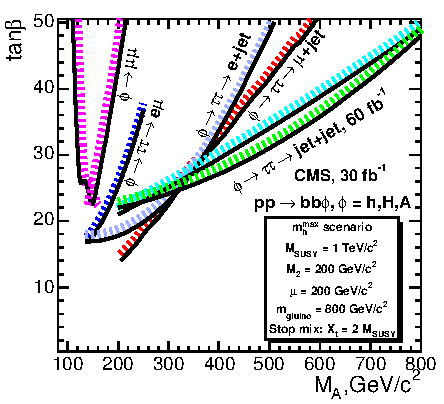
\includegraphics[width=0.65\textwidth]{analysis/discovery_hneutral}
\caption{5$\sigma$ reach in the \plane plane in the \mhmax scenario. Both this analysis (the green line) and the b-tagging analysis (cyan line) are shown for 60 \fb. The area above a line is reachable in that channel. ~\cite{CMS_TDR_PHYS_vol2} \label{fig:discovery}}
\end{figure}

Replacing the b-tagging event selection with an \MET cut resulted in improved $\tan{\beta}$ sensitivity for $m_{A} =$ 500 and 800\GeVcc. However at low values ($m_{A} \approx 200 \GeVcc$) the amount of \MET in signal and background events was similar. This resulted in a cut that removed a significant amount of the signal ($\sim 90\%$). At the highest values of $m_{A} \approx 800 \GeVcc$  the low number of signal events and the large background uncertainty reduced the sensitivity.

%\section{comparison to previous study}
%LEP, Tevatron, b-tagg sasha

\section{Conclusion}
It was concluded that CMS was sensitive to the MSSM heavy Higgs boson in the range 200\,$<$\,$m_{A}$\,$<$\,800\GeVcc with $\tan{\beta}$\,$\ge$\,48. This was slightly better than the previous b-tagging study except at $m_{A}$\,=\,200\GeVcc. 

When this analysis is performed on real data it will be combined with the b-tagging study to obtain the greatest reach. The other channels shown in Figure~\ref{fig:discovery} will also be combined with the aim of providing the greatest possible reach. These will be combined with general MSSM searches to perform a fit of the MSSM parameter space.

Any improvement in the \MET performance of the CMS experiment would benefit this channel. It is likely that both the \MET scale and resolution will be improved when CMS implements energy flow. This would increase reach in the \plane plane especially for $m_{A} \approx 200 \GeVcc$.